\documentclass[11pt]{article}
\usepackage[margin=1in]{geometry}
\usepackage{hyperref}
\usepackage{graphicx}
\graphicspath{{../../shared/figures/}}
\usepackage{natbib}
\bibliographystyle{unsrtnat}
\usepackage{doi}
% \setcitestyle{numbers,super} % Superscript citation numbers (e.g. ¹, ²⁻⁴) — does not support locator notes
\setcitestyle{numbers,square} % Square brackets around citation numbers (e.g. [1], [2-4]) — math standard
% ── Merge citation text into a single hyperlink ───────────────────────────────
\makeatletter
\renewcommand{\hyper@natlinkbreak}[2]{#1}
\makeatother
\usepackage{titlesec}
% New page before each top-level section
% \newcommand{\sectionbreak}{\clearpage}

% ── Theorem-like environments ─────────────────────────────────────────────────
\usepackage{amsmath}
\usepackage{amsthm}
\usepackage{thmtools}
\declaretheorem[name=Theorem]{theorem}
\declaretheorem[name=Proposition,sibling=theorem]{proposition}
\declaretheorem[name=Lemma,sibling=theorem]{lemma}
\declaretheorem[name=Corollary,sibling=theorem]{corollary}
\declaretheorem[name=Conjecture,sibling=theorem]{conjecture}

\theoremstyle{definition}
\declaretheorem[name=Definition,style=definition]{definition}
\declaretheorem[name=Axiom,style=definition,sibling=definition]{axiom}
\declaretheorem[name=Assumption,style=definition,sibling=definition]{assumption}
\declaretheorem[name=Criterion,style=definition,sibling=definition]{criterion}
\declaretheorem[name=Example,style=definition,sibling=definition]{example}

\theoremstyle{remark}
\declaretheorem[name=Remark,style=remark]{remark}
\declaretheorem[name=Observation,style=remark,sibling=remark]{observation}
\declaretheorem[name=Property,style=remark,sibling=remark]{property}

% Prevent theorem-like environments from starting near the page bottom.
\usepackage{etoolbox}
\BeforeBeginEnvironment{theorem}{\needspace{4\baselineskip}\addvspace{6pt}}
\BeforeBeginEnvironment{corollary}{\needspace{4\baselineskip}\addvspace{6pt}}
\BeforeBeginEnvironment{lemma}{\needspace{4\baselineskip}\addvspace{6pt}}
\BeforeBeginEnvironment{proposition}{\needspace{4\baselineskip}\addvspace{6pt}}
\BeforeBeginEnvironment{definition}{\needspace{4\baselineskip}\addvspace{6pt}}
\BeforeBeginEnvironment{axiom}{\needspace{4\baselineskip}\addvspace{6pt}}
\BeforeBeginEnvironment{assumption}{\needspace{4\baselineskip}\addvspace{6pt}}
\BeforeBeginEnvironment{remark}{\needspace{4\baselineskip}\addvspace{9pt}}

% ── Pandoc-generated table support ────────────────────────────────────────────
\usepackage{longtable}
\usepackage{booktabs}
\usepackage{array}
\usepackage{calc}
\usepackage{caption}
% Pandoc 3.x wraps uncaptioned longtables in \def\LTcaptype{none};
% this requires a 'none' counter to exist.
\newcounter{none}

% ── Paragraph spacing (matches Pandoc default) ────────────────────────────────
% No paragraph indentation; inter-paragraph spacing instead.
\usepackage{parskip}

% ── Page-break quality ────────────────────────────────────────────────────────
% Prevent widow/orphan lines (single line stranded at top/bottom of page).
\widowpenalty=10000
\clubpenalty=10000
% Pin footnotes to the page bottom even with \raggedbottom.
\usepackage[bottom]{footmisc}
% Prevent page breaks immediately before or after display equations.
\predisplaypenalty=10000
\postdisplaypenalty=150
% Allow uneven page bottoms rather than stretching vertical glue.
\raggedbottom
% Increase separation between body text and footnotes.
\setlength{\skip\footins}{1.5\baselineskip}
% Ensure headings don't appear at page bottom without body text following.
\usepackage{needspace}
% Reserve enough space for the heading itself plus at least two following
% lines of body text (or a nested heading plus a line). This prevents a
% heading from appearing at the bottom of a page with its content (or its
% next-level subheading) starting on the following page.
\let\origsection\section
\renewcommand{\section}{\needspace{8\baselineskip}\origsection}
\let\origsubsection\subsection
\renewcommand{\subsection}{\needspace{8\baselineskip}\origsubsection}
\let\origsubsubsection\subsubsection
\renewcommand{\subsubsection}{\needspace{6\baselineskip}\origsubsubsection}
\let\origparagraphcmd\paragraph
\renewcommand{\paragraph}{\needspace{4\baselineskip}\origparagraphcmd}
\let\origsubparagraph\subparagraph
\renewcommand{\subparagraph}{\needspace{4\baselineskip}\origsubparagraph}

% Discourage page breaks inside multi-line math environments (align, gather, etc.)
\interdisplaylinepenalty=10000

% ── Section numbering ────────────────────────────────────────────────────────
% Pandoc --number-sections generates \section{...} (not \section*{...}).
% LaTeX auto-numbers to depth 3 (subsubsection) by default.
\setcounter{secnumdepth}{3}

% ── Make \paragraph and \subparagraph block-level (matches Pandoc) ───────────
% By default LaTeX renders \paragraph as a run-in heading (text continues on
% the same line). These commands make them free-standing headings with
% proper spacing before and after.
\titleformat{\paragraph}
  {\normalfont\normalsize\bfseries}{\theparagraph}{1em}{}
\titlespacing*{\paragraph}
  {0pt}{3.25ex plus 1ex minus .2ex}{1.5ex plus .2ex}
\titleformat{\subparagraph}
  {\normalfont\normalsize\bfseries}{\thesubparagraph}{1em}{}
\titlespacing*{\subparagraph}
  {0pt}{3.25ex plus 1ex minus .2ex}{1.5ex plus .2ex}

% ── Pandoc-generated tightlist support ────────────────────────────────────────
\providecommand{\tightlist}{%
  \setlength{\itemsep}{0pt}\setlength{\parskip}{0pt}}

% ── Pandoc 3.x figure sizing ─────────────────────────────────────────────────
% \pandocbounded constrains included graphics to text width when they exceed it
\newcommand{\pandocbounded}[1]{%
  \sbox0{#1}%
  \ifdim\wd0>\linewidth
    \resizebox{\linewidth}{!}{#1}%
  \else
    #1%
  \fi
}

% ── Unicode character fixes ───────────────────────────────────────────────────
\usepackage{amssymb}
\usepackage{newunicodechar}
\newunicodechar{✓}{$\checkmark$}
\newunicodechar{≠}{$\neq$}
\newunicodechar{≡}{$\equiv$}
\newunicodechar{≈}{$\approx$}
\newunicodechar{δ}{$\delta$}
\newunicodechar{−}{$-$}
% Superscript digits used in scientific notation (e.g. 10^-7, 10^29)
\newunicodechar{⁰}{$^{0}$}
% ¹²³ already defined by textcomp; suppress redefinition warning
\begingroup\renewcommand\PackageWarning[2]{}%
\newunicodechar{¹}{$^{1}$}
\newunicodechar{²}{$^{2}$}
\newunicodechar{³}{$^{3}$}
\endgroup
\newunicodechar{⁴}{$^{4}$}
\newunicodechar{⁵}{$^{5}$}
\newunicodechar{⁶}{$^{6}$}
\newunicodechar{⁷}{$^{7}$}
\newunicodechar{⁸}{$^{8}$}
\newunicodechar{⁹}{$^{9}$}
\newunicodechar{⁻}{$^{-}$}
% Fix \rightarrow for use outside math mode
\let\mystRightarrow\rightarrow
\renewcommand{\rightarrow}{\ensuremath{\mystRightarrow}}
% ─────────────────────────────────────────────────────────────────────────────

% Allow TeX extra stretch to resolve moderate overfull hboxes
\emergencystretch=2em

\hypersetup{colorlinks=true, allcolors=blue}

\title{Thermodynamics of Cooperation: Accumulated Negentropy}
\author{Keith Lostracco}
\date{}

\begin{document}
\maketitle

\begin{abstract}
Complex dissipative structures, from ecosystems to biospheres, embody
thermodynamic investments accumulated over evolutionary timescales. The
quantitative magnitude of this investment, and the sustainability limits
it imposes, have not been derived from first principles. We define
accumulated negentropy as the integrated thermodynamic work invested in
a system's information content over its history and, using Landauer's
principle as the thermodynamic floor, provide a biosphere-scale
accounting of this quantity. Earth's biosphere embodies \(\sim 10^{29}\)
J of accumulated negentropy, a value cross-validated within a factor of
1.36 using independent energy rate density measurements. The
Burning-Library Ratio \(\mathcal{R}_{\text{BL}} \approx 10^{-7}\)
quantifies a seven-order-of-magnitude gap between the energy recoverable
through destruction and the thermodynamic cost of replacement. We
formalize the coupling between a system's accumulated complexity and its
generative information rate, proving that partial destruction incurs a
superlinear penalty on future information production. This rate-stock
coupling yields four applied results: (1) a tipping-point threshold
below which complex systems collapse irreversibly, consistent with the
observed 20-25\% deforestation threshold for the Amazon; (2) a maximum
sustainable extraction bound derived from the balance between generative
and decay rates; (3) superlinear recovery times that explain the
observed hierarchy from fast-recovering grasslands to
threshold-dominated rainforests; and (4) a conservation fidelity bound
showing that ex-situ archives cannot substitute for in-situ
preservation. The framework provides computable, energy-denominated
sustainability limits for any complex dissipative structure whose
information content was produced by extended search. The analysis
requires only Landauer's principle, basic thermodynamics, and
order-of-magnitude estimates from astrophysics and biology.
\end{abstract}
\newpage
\tableofcontents
\newpage
\section{Introduction}\label{introduction}

Complex dissipative structures, from individual organisms to entire
biospheres, persist by continuously importing free energy and exporting
entropy to maintain their internal order. That this ordering work is
irreversible, and that complex systems embody thermodynamic investments
far exceeding any energy recoverable from their raw materials, is
qualitatively well understood. Less explored is the quantitative
question: how large is the thermodynamic investment embodied in
biological complexity, and what sustainability limits does that
investment impose? This paper provides that accounting.

We define \emph{accumulated negentropy} as the integrated thermodynamic
work invested in a system's information content over its history
(Definition~\ref{def-accumulated-negentropy}). Using Landauer's
principle \citep{Landauer1961} as the absolute thermodynamic floor for
information creation, we establish a hierarchy of results:

\begin{enumerate}
\def\labelenumi{\arabic{enumi}.}
\tightlist
\item
  Rebuilding a complex system by blind search costs at least as much as
  the original evolutionary investment
  (Theorem~\ref{thm-minimum-replication-cost}), estimated at
  \(\sim 10^{29}\) J for Earth's biosphere, cross-validated within a
  factor of 1.36 using independent energy rate density measurements from
  \citep{Chaisson2011}.
\item
  The Burning-Library Ratio (Definition~\ref{def-burning-library-ratio})
  quantifies a seven-order-of-magnitude gap between the energy
  recoverable from the biosphere's raw materials and its accumulated
  thermodynamic investment: the recoverable fraction is approximately
  \(10^{-7}\) (Theorem~\ref{thm-irrationality-destruction}).
\item
  Living systems produce new information at a positive rate whose
  present value is finite for any positive time-preference rate but
  grows without bound as the planning horizon extends
  (Theorem~\ref{thm-present-value-generative-info}); at conventional
  ecological discount rates, biosphere-scale parameters yield
  \(PV_{\text{gen}} \sim 10^{14}\) to \(10^{22}\) J
  (Corollary~\ref{cor-generative-pv-bound}).
\end{enumerate}

The rate-stock coupling between accumulated complexity and generative
information rate (Definition~\ref{def-rate-stock-coupling}) yields
further results: a tipping-point threshold below which systems collapse
irreversibly (Proposition~\ref{prop-negentropy-tipping-point}), a
maximum sustainable extraction bound
(Corollary~\ref{cor-maximum-sustainable-extraction}), superlinear
recovery times that explain the observed hierarchy from fast-recovering
grasslands to threshold-dominated rainforests
(Proposition~\ref{prop-superlinear-recovery-time}), and a conservation
fidelity bound showing that ex-situ archives cannot substitute for
in-situ preservation
(Proposition~\ref{prop-conservation-fidelity-bound}).

The results connect to the multi-agent dissipative optimization models
developed in \emph{Necessary Constraints} \citep{TC-I} and
\emph{Thermodynamic Friction} \citep{TC-IV}; the core argument requires
only Landauer's principle, basic thermodynamics, and order-of-magnitude
estimates from astrophysics and biology.

The paper proceeds as follows: model and formal setup, information
density and the Landauer floor, accumulated negentropy and the
entropy-maintenance inequality, biosphere estimation with
cross-validation against Chaisson's energy rate density, replication
cost, the thermodynamic cost-benefit analysis (Burning-Library Ratio,
rate-stock coupling, tipping points, sustainable extraction, recovery
times, conservation fidelity), synthesis into the cross-scale
sustainability theorem, worked examples, and discussion.

\subsection{Related Work}\label{related-work}

\subsubsection{Information as Physical}\label{information-as-physical}

The century-long resolution of Maxwell's Demon established that
information is physical. \citet{Szilard1929} showed that measurement
produces at least \(k_B \ln 2\) of entropy per bit.
\citeauthor{Brillouin1951}
\citetext{\citeyear{Brillouin1951}; \citeyear{Brillouin1962}} proved the
formal equivalence between Shannon information and thermodynamic entropy
via \(S_{\text{info}} = k_B \ln 2 \cdot H(X)\). \citet{Landauer1961}
identified erasure as the irreducible cost: erasing one bit at
temperature \(T\) dissipates at least \(k_B T \ln 2\) joules, a result
experimentally verified by \citet{Berut2012}. \citeauthor{Bennett1973}
\citetext{\citeyear{Bennett1973}; \citeyear{Bennett1982}} completed the
resolution by demonstrating that measurement can be reversible; only
erasure carries unavoidable entropy cost.

This physical grounding of information establishes the thermodynamic
floor for every result in this paper: the cost of creating, maintaining,
or destroying one bit of information has an irreducible energy component
set by the laws of physics, not by technology or computational
sophistication.

\subsubsection{Information Content of Biological
Systems}\label{information-content-of-biological-systems}

\citet{Adami2004} proved that Shannon entropy rigorously measures the
information content of biological sequences, with each round of natural
selection reducing genomic entropy and accumulating mutual information
between organisms and environments. \citet{Chaisson2011} introduced
energy rate density \(\Phi_m\) as a cross-scale complexity metric,
demonstrating that biological systems achieve orders-of-magnitude higher
values than non-biological systems. \citet{Schrodinger1944} first
characterized living organisms as negative-entropy systems that maintain
internal order by extracting free energy from their environment.

To our knowledge, Landauer's principle has not previously been applied
at the biosphere scale (\(\sim 10^{15}\) functional bits accumulated
over \(4 \times 10^9\) years) to compute the total thermodynamic
investment embodied in biological complexity and to derive the
sustainability limits this investment imposes. We perform this
integration and quantify the resulting cost-benefit gap at approximately
seven orders of magnitude.

\subsubsection{The Gap}\label{the-gap}

The information-theoretic tradition established that information is
quantifiable \citep{Shannon1948}, physical
\citep{Brillouin1962, Landauer1961}, and accumulates through evolution
\citep{Adami2004}. Complexity increases over cosmic time
\citep{Chaisson2011}. What the tradition left unresolved was the formal
connection between a system's accumulated thermodynamic investment and
its dynamic properties: how the total ordering work invested over
evolutionary time determines the system's generative capacity, its
fragility to partial damage, and the timescales required for recovery.
This paper formalizes that connection and derives the resulting bounds.

\section{Model and Formal Setup}\label{model-and-formal-setup}

We consider physical systems that maintain internal order by dissipating
free energy, within the multi-agent framework of \citep{TC-I}. The
analysis requires three assumptions.

\begin{assumption}[Second Law and Irreversibility]
\label{asm-second-law}

All systems obey the Second Law of thermodynamics: the total entropy of an isolated system does not decrease. Maintaining internal order (low entropy) requires continuous thermodynamic work. When that work ceases, the system's entropy increases toward the maximum-entropy (thermal equilibrium) state.
\end{assumption}

\begin{assumption}[Landauer's Principle]
\label{asm-landauer-principle}

Erasing (or creating) one bit of information at temperature $T$ requires a minimum energy expenditure of $k_B T \ln 2$ joules, where $k_B \approx 1.381 \times 10^{-23}$ J/K is Boltzmann's constant \citep{Landauer1961}. This bound is the absolute thermodynamic floor; real physical processes operate far above it.
\end{assumption}

\begin{assumption}[Functional Information]
\label{asm-functional-information}

The information content of biological systems consists of \emph{functional} configurations selected by evolutionary processes. A random configuration of equivalent length is overwhelmingly unlikely to be functional. The fraction of functional configurations in the relevant state space satisfies $f_{\text{func}} \ll 1$.
\end{assumption}

The central quantity of this work is \emph{accumulated negentropy}: the
integrated thermodynamic work invested in a system's information content
over its history, defined precisely in
§\ref{accumulated-negentropy-the-time-integral-of-order}. The
information-theoretic formalism (information density, Shannon and
Boltzmann entropy, and the Brillouin-Landauer bridge connecting them) is
developed in §\ref{information-density-negentropy-as-value}.

\begin{remark}[Nature of the quantitative results]
\label{rem-order-of-magnitude}

The quantitative results, notably the estimates of biosphere accumulated negentropy ($\sim 10^{29}$ J), the Burning-Library Ratio ($\sim 10^{-7}$), and the search cost amplification factor ($\sim 10^{35}$), are order-of-magnitude bounds derived from empirical inputs (photosynthetic capture rates, biomass inventories, genome sizes) that are individually uncertain by factors of 2 to 10. We state all such results with the $\sim$ qualifier and treat them as order-of-magnitude estimates throughout. The formal results (Theorem~\ref{thm-irrationality-destruction}, Theorem~\ref{thm-negentropy-defense}) are exact given their inputs; it is the inputs that carry uncertainty. The central conclusion, that the thermodynamic gap between destruction yield and accumulated investment spans approximately seven orders of magnitude, is robust to factor-of-$10^3$ uncertainties in any single input: the gap would have to close by seven full orders of magnitude to alter the qualitative result. See §\ref{limitations} for a detailed discussion of sensitivity.
\end{remark}

\section{Information Density: Negentropy as
Value}\label{information-density-negentropy-as-value}

\subsection{Motivation: Why Raw Energy ≠
Value}\label{motivation-why-raw-energy-value}

A star has enormous raw energy but minimal informational structure
(burning plasma), while a forest has modest energy but extraordinary
\textbf{information density}, billions of years of evolutionary
trial-and-error encoded in DNA, neural circuits, and ecosystem
interdependencies. If ``value'' to the broader network were measured
only by instantaneous energy, a single fusion reactor would outweigh the
entire biosphere. The corrective is to measure value not by
instantaneous energy but by \textbf{informational complexity}, the
degree to which a system has organized matter against entropy. This
section formalizes that notion.

\subsection{Thermodynamic Entropy and
Microstates}\label{thermodynamic-entropy-and-microstates}

A physical system with \(\Omega\) equally accessible microstates has
\textbf{Boltzmann entropy}:

\[S = k_B \ln \Omega\]

where \(k_B \approx 1.381 \times 10^{-23}\) J/K is Boltzmann's constant.
For a general probability distribution over microstates
\(\{p_m\}_{m=1}^{\Omega}\):

\[S = -k_B \sum_{m=1}^{\Omega} p_m \ln p_m\]

The maximum-entropy state (thermal equilibrium) has \(p_m = 1/\Omega\)
for all \(m\), giving \(S_{\max} = k_B \ln \Omega\).

\subsection{Shannon Entropy as Informational
Entropy}\label{shannon-entropy-as-informational-entropy}

Shannon's entropy for a discrete random variable \(X\) with probability
mass function \(\{p(x)\}\) is:

\[H(X) = -\sum_{x} p(x) \log_2 p(x) \quad \text{(bits)}\]

The connection to thermodynamic entropy is established by the
\textbf{Brillouin-Landauer bridge}:

\[S_{\text{info}} = k_B \ln 2 \cdot H(X) \quad \text{(J/K)}\]

Every bit of information is equivalent to \(k_B \ln 2\) units of
thermodynamic entropy. Erasing one bit of information \textbf{must}
dissipate at least \(k_B T \ln 2\) joules of heat (Landauer's
principle).

\subsection{Information Density: Formal
Definition}\label{information-density-formal-definition}

\begin{definition}[Information Density]
\label{def-information-density}

The \textbf{information density} of a physical system is the difference between its maximum-entropy state and its actual thermodynamic entropy:

$$\mathcal{I} \triangleq S_{\max} - S_{\text{actual}} \geq 0$$

Equivalently, in information-theoretic units (bits):

$$\mathcal{I}_{\text{bits}} = \frac{S_{\max} - S_{\text{actual}}}{k_B \ln 2} = H_{\max}(X) - H(X) \geq 0$$

where $H_{\max}(X) = \log_2 |\mathcal{X}|$ is the maximum entropy over the state space $\mathcal{X}$.
\end{definition}

\textbf{Interpretation:} \(\mathcal{I}\) is the \textbf{negentropy} of
the system \citep{Brillouin1962}, the amount by which the system is
\emph{more ordered} than its thermal equilibrium. A system at thermal
equilibrium (\(S = S_{\max}\)) has \(\mathcal{I} = 0\): no information,
no structure, no complexity. A highly ordered system (a living organism,
a crystal, a computer memory) has \(\mathcal{I} \gg 0\): it carries
significant information that distinguishes it from random thermal noise.

\begin{definition}[Specific Information Density]
\label{def-specific-information-density}

The \textbf{specific information density} of a system is the information density per unit mass:

$$\rho_{\mathcal{I}} \triangleq \frac{\mathcal{I}_{\text{bits}}}{m} \quad \text{(bits/kg)}$$

where $m$ is the system's mass. This enables cross-scale comparisons: a star has very low $\rho_{\mathcal{I}}$ (simple structure, enormous mass); a human genome has very high $\rho_{\mathcal{I}}$ (complex structure, tiny mass).
\end{definition}

\subsection{Landauer's Principle: The Thermodynamic Floor of
Information}\label{landauers-principle-the-thermodynamic-floor-of-information}

\begin{theorem}[Landauer's Bound: Minimum Cost of Information Erasure]
\label{thm-landauer-bound}

Erasing (or equivalently, creating from random noise) one bit of information in a system at temperature $T$ requires a minimum energy expenditure of:

$$E_{\text{Landauer}} = k_B T \ln 2 \approx 2.87 \times 10^{-21} \text{ J at } T = 300\text{ K}$$

Therefore, creating a system with information density $\mathcal{I}_{\text{bits}}$ from maximally disordered matter requires at minimum:

$$W_{\text{create}}^{\min} = \mathcal{I}_{\text{bits}} \cdot k_B T \ln 2$$
\end{theorem}

\begin{proof}
(Sketch.) @Landauer1961 showed that logically irreversible operations (such as resetting a bit to a known state) must increase the entropy of the environment by at least $k_B \ln 2$ per bit. Creating one bit of order (reducing entropy by $k_B \ln 2$) in a subsystem requires expelling at least $k_B T \ln 2$ of heat into the environment at temperature $T$, by the Second Law. The result follows by linearity for $\mathcal{I}_{\text{bits}}$ independent bits.
\end{proof}

\textbf{Critical caveat:} Landauer's bound is the absolute thermodynamic
\textbf{floor}, the minimum energy if every operation is performed with
perfect thermodynamic efficiency. Real physical processes operate far
above this floor (biological systems operate at \(\xi \approx 10^5\) to
\(10^8\) times the Landauer limit per bit; see \citep{TC-II}). The
actual cost of creating complex biological structures dwarfs the
Landauer bound by many orders of magnitude, a point that is essential to
the argument below.

\section{Accumulated Negentropy: The Time-Integral of
Order}\label{accumulated-negentropy-the-time-integral-of-order}

\subsection{Motivation: Complexity Requires Sustained
Work}\label{motivation-complexity-requires-sustained-work}

A living system does not appear instantaneously. Its information density
\(\mathcal{I}(t)\) is the result of a continuous process (evolution,
self-organization, learning) during which thermodynamic work is invested
in selecting, testing, and preserving ordered configurations against
entropic decay. The \textbf{instantaneous} information density
\(\mathcal{I}(t)\) at time \(t\) tells us the \emph{current} order; but
the true ``cost'' of producing that order is the \emph{entire history}
of thermodynamic investment.

Consider: a random recombination that produces the same DNA sequence as
a human genome would have the same instantaneous \(\mathcal{I}\) but
would be astronomically unlikely (and energetically cheap to destroy,
since no selection process maintains it). The difference lies in the
\textbf{accumulated work} that natural selection invested to discover,
refine, and stabilize that sequence over billions of years.

\subsection{The Formal Definition}\label{the-formal-definition}

\begin{definition}[Accumulated Negentropy]
\label{def-accumulated-negentropy}

The \textbf{accumulated negentropy} of a system at time $T$ is the total thermodynamic work invested over the system's history in creating and maintaining its current information density:

$$\mathcal{N}(T) \triangleq \int_0^T \dot{W}_{\text{order}}(t) \, dt$$

where $\dot{W}_{\text{order}}(t)$ is the instantaneous rate of thermodynamic work directed toward \textbf{entropy reduction} (ordering) at time $t$, measured in watts (J/s).
\end{definition}

\textbf{Decomposition:} The ordering work rate has two components:

\[\dot{W}_{\text{order}}(t) = \dot{W}_{\text{construct}}(t) + \dot{W}_{\text{maintain}}(t)\]

\begin{definition}[Construction Work]
\label{def-construction-work}

$\dot{W}_{\text{construct}}(t)$ is the rate of thermodynamic work that \emph{increases} the system's information density (building new structures, evolving new genes, forming new neural connections).
\end{definition}

\begin{definition}[Maintenance Work]
\label{def-maintenance-work}

$\dot{W}_{\text{maintain}}(t)$ is the rate of thermodynamic work that \emph{preserves} existing information density against entropic decay (repairing DNA, maintaining cell membranes, fighting infection).
\end{definition}

The Second Law requires \(\dot{W}_{\text{maintain}}(t) > 0\) for all
\(t\) at which the system exists: if maintenance work ceases, entropy
floods in and the information density decays. This is the thermodynamic
basis of mortality; death is the cessation of maintenance work.

\subsection{The Entropy-Maintenance
Inequality}\label{the-entropy-maintenance-inequality}

\begin{proposition}[Minimum Maintenance Work]
\label{prop-minimum-maintenance-work}

A system with information density $\mathcal{I}(t)$ at temperature $T$ in an environment with entropy injection rate $\dot{S}_{\text{env}}(t)$ must perform maintenance work at a rate of at least:

$$\dot{W}_{\text{maintain}}(t) \geq T \cdot \dot{S}_{\text{env}}(t)$$

to prevent net entropy increase (information loss). Equivalently, in bits:

$$\dot{W}_{\text{maintain}}(t) \geq k_B T \ln 2 \cdot \dot{H}_{\text{decay}}(t)$$

where $\dot{H}_{\text{decay}}(t)$ is the rate at which information would be lost (in bits/s) if no maintenance were performed.
\end{proposition}

\begin{proof}
By the Second Law, the system's total entropy change is $dS/dt = \dot{S}_{\text{env}} - \dot{S}_{\text{export}}$, where $\dot{S}_{\text{export}}$ is the entropy exported via waste heat. To maintain $S \leq S_{\text{actual}}$ (no information loss), the system must export entropy at a rate $\dot{S}_{\text{export}} \geq \dot{S}_{\text{env}}$. By the Clausius inequality, exporting entropy $\dot{S}_{\text{export}}$ at temperature $T$ requires work $\dot{W} \geq T \cdot \dot{S}_{\text{export}} \geq T \cdot \dot{S}_{\text{env}}$. The bit-denominated version follows from $\Delta S = k_B \ln 2 \cdot \Delta H$.
\end{proof}

\subsection{The Accumulation Equation}\label{the-accumulation-equation}

The system's information density evolves as:

\[\frac{d \mathcal{I}}{dt} = \frac{d \mathcal{I}_{\text{bits}}}{dt} = \underbrace{r_{\text{construct}}(t)}_{\text{new order creation}} - \underbrace{r_{\text{decay}}(t)}_{\text{entropy erosion}} + \underbrace{r_{\text{maintain}}(t)}_{\text{maintenance recovery}}\]

where: - \(r_{\text{construct}}(t)\) = bits/s of new information created
(e.g., advantageous mutations fixed, new neural connections formed) -
\(r_{\text{decay}}(t)\) = bits/s of entropic erosion pressure on
existing information (gross decay rate before maintenance) -
\(r_{\text{maintain}}(t)\) = bits/s of information that \emph{would have
decayed} but was saved by maintenance work

For a surviving system (one whose information density does not
decrease), the condition
\(r_{\text{construct}} + r_{\text{maintain}} \geq r_{\text{decay}}\)
must hold at all times. Note that by definition
\(r_{\text{maintain}} \leq r_{\text{decay}}\) (maintenance cannot
prevent more decay than exists). When maintenance fully compensates
decay (\(r_{\text{maintain}} = r_{\text{decay}}\)), a system whose
complexity is \textbf{growing} (evolution, learning) satisfies:

\[\frac{d \mathcal{I}_{\text{bits}}}{dt} \geq r_{\text{construct}}(t) > 0\]

and therefore \(\mathcal{I}_{\text{bits}}(T)\) is an increasing function
of time. The accumulated negentropy captures both the construction and
the maintenance:

\[\mathcal{N}(T) = \underbrace{\int_0^T \dot{W}_{\text{construct}}(t) \, dt}_{\mathcal{N}_{\text{construct}}} + \underbrace{\int_0^T \dot{W}_{\text{maintain}}(t) \, dt}_{\mathcal{N}_{\text{maintain}}}\]

\section{Biosphere Estimation: The 4-Billion-Year
Ledger}\label{biosphere-estimation-the-4-billion-year-ledger}

\subsection{The Approach}\label{the-approach}

We estimate Earth's biosphere accumulated negentropy using two
complementary methods:

\begin{enumerate}
\def\labelenumi{\arabic{enumi}.}
\tightlist
\item
  \textbf{Top-down (energy input):} How much solar energy has been
  captured and channeled into biological ordering work?
\item
  \textbf{Bottom-up (information content):} How many bits of functional
  information does the biosphere contain, and what is the minimum energy
  required to produce that information?
\end{enumerate}

The two estimates bracket the true value: the top-down gives an upper
bound (not all captured energy goes to ordering), and the bottom-up
gives a lower bound (the Landauer floor underestimates real construction
costs by many orders of magnitude).

\subsection{Top-Down: Solar Energy Captured by the
Biosphere}\label{top-down-solar-energy-captured-by-the-biosphere}

\textbf{Step 1: Solar power intercepted by Earth.}

The total solar irradiance at Earth's orbit is
\(\mathcal{S}_0 \approx 1361\) W/m² \citep{Burch2021}. Earth's
cross-sectional area is \(A_E = \pi R_E^2\) with
\(R_E \approx 6.371 \times 10^6\) m:

\[P_{\text{solar}} = \mathcal{S}_0 \cdot \pi R_E^2 \approx 1361 \times 1.275 \times 10^{14} \approx 1.735 \times 10^{17} \text{ W}\]

\textbf{Step 2: Photosynthetic capture.}

Gross primary production (GPP), the total power captured by
photosynthesis globally, is estimated at:

\[P_{\text{GPP}} \approx 1.5 \times 10^{14} \text{ W}\]

(based on \textasciitilde{}\(1.2 \times 10^{17}\) gC/yr fixed by
photosynthesis at \textasciitilde{}\(4 \times 10^4\) J/gC; see
\citeyearpar{Beer2010}). This is approximately 0.087\% of the total
intercepted solar power, consistent with standard estimates of global
photosynthetic efficiency \citeyearpar{Beer2010}.

\textbf{Step 3: Fraction directed to ordering work.}

Not all captured energy creates or maintains biological order. Most is
used for basal metabolism (heat generation). Growth respiration (the
energetic cost of synthesizing new biomass) constitutes roughly 25--30\%
of total autotrophic respiration \citep{Smil2002}, but only a fraction
of new biomass encodes novel information; the remainder is bulk
structural material (cellulose, lignin). We use a conservative ordering
efficiency \(\eta_{\text{order}} \approx 0.01\) (1\% of GPP):

\[\dot{W}_{\text{order}} \approx \eta_{\text{order}} \cdot P_{\text{GPP}} \approx 0.01 \times 1.5 \times 10^{14} = 1.5 \times 10^{12} \text{ W}\]

\textbf{Step 4: Time integration.}

The biosphere has existed for \(T_{\text{bio}} \approx 4 \times 10^9\)
years \(= 4 \times 10^9 \times 3.156 \times 10^7\) s
\(\approx 1.26 \times 10^{17}\) s.

Assuming \(\dot{W}_{\text{order}}\) scales roughly linearly from
near-zero (early microbial life) to its present value (an average of
approximately half the current rate over the full interval):

\[\mathcal{N}_{\text{bio}}^{\text{top-down}} \approx \frac{1}{2} \dot{W}_{\text{order}}^{\text{now}} \cdot T_{\text{bio}} \approx \frac{1}{2} \times 1.5 \times 10^{12} \times 1.26 \times 10^{17} \approx 9.45 \times 10^{28} \text{ J}\]

\begin{quote}
\textbf{Estimate 1 (Top-Down Accumulated Negentropy).}

\[\mathcal{N}_{\text{bio}}^{\text{top-down}} \sim 10^{29} \text{ J}\]
\end{quote}

\textbf{Order-of-magnitude check:} The total solar energy intercepted by
Earth over 4 Gyr is
\(P_{\text{solar}} \times T_{\text{bio}} \approx 1.735 \times 10^{17} \times 1.26 \times 10^{17} \approx 2.2 \times 10^{34}\)
J. Our estimate uses only a fraction \(\sim 10^{29}/10^{34} = 10^{-5}\)
of total intercepted solar energy. This is physically plausible: most
solar energy drives weather, heats the surface, and is re-radiated as
thermal infrared. Only a tiny fraction organizes matter against entropy.

\subsection{Bottom-Up: Information Content of the
Biosphere}\label{bottom-up-information-content-of-the-biosphere}

\textbf{Step 1: Information content of a single genome.}

The human genome contains approximately \(3.2 \times 10^9\) base pairs.
Each base pair encodes 2 bits of information (4 possible nucleotides):

\[H_{\text{genome}}^{\text{raw}} = 3.2 \times 10^9 \times 2 = 6.4 \times 10^9 \text{ bits} \approx 6.4 \text{ Gbits}\]

However, due to redundancy (non-coding regions, repeated sequences), the
\textbf{functional information content} is lower. Estimates of
functional sequence range from 5\% \citep{Kellis2014} to 15\%
\citep{Graur2017} of the genome:

\[H_{\text{genome}}^{\text{functional}} \approx 0.10 \times 6.4 \times 10^9 = 6.4 \times 10^8 \text{ bits} \approx 640 \text{ Mbits}\]

\textbf{Step 2: Information content of the entire biosphere.}

Estimated number of species on Earth:
\(N_{\text{species}} \sim 8.7 \times 10^6\) \citep{Mora2011}. Few
species share identical genomes; the average inter-species genomic
divergence contributes significant unique information. Conservatively,
each species contributes at least \(\sim 10^7\) bits of unique
functional information (after accounting for shared evolutionary
heritage):

\[H_{\text{biosphere}}^{\text{genetic}} \approx N_{\text{species}} \times 10^7 \approx 8.7 \times 10^{13} \text{ bits}\]

\textbf{Alternative estimate via raw genomic sequence.} Genome sizes
range from \(\sim 4 \times 10^6\) bp in bacteria to \(\sim 10^{10}\) bp
in large eukaryotes, with a geometric mean across all life of roughly
\(10^8\)--\(10^9\) bp \citep{Milo2015}. At 2 bits per base pair
\citep{Adami2004}:

\[H_{\text{biosphere}}^{\text{raw}} \approx 8.7 \times 10^6 \times (2 \times 10^8 \text{–} 2 \times 10^9) \sim 10^{15} \text{ bits}\]

The two paths bracket the estimate: the functional-information route
(\(\sim 10^{14}\) bits, counting only unique non-redundant sequence)
provides a lower bound, while the raw-sequence route (\(\sim 10^{15}\)
bits) provides an upper bound. Additional information layers
(\textbf{epigenetic}: methylation patterns and histone modifications;
\textbf{connectomic}: neural wiring; \textbf{ecological}: species
interaction networks and ecosystem structures) contribute further bits
that close the gap from below. Both estimates agree at order of
magnitude:

\[H_{\text{biosphere}}^{\text{total}} \sim 10^{15} \text{ bits} = 1 \text{ Pbit (petabit)}\]

\textbf{Step 3: Landauer floor for this information.}

At \(T = 300\) K:

\[W_{\text{Landauer}}^{\text{bio}} = H_{\text{biosphere}}^{\text{total}} \times k_B T \ln 2 = 10^{15} \times 2.87 \times 10^{-21} \approx 2.87 \times 10^{-6} \text{ J}\]

\begin{quote}
\textbf{Estimate 2 (Landauer Floor of Biosphere Information).}

\[W_{\text{Landauer}}^{\text{bio}} \sim 10^{-6} \text{ J}\]
\end{quote}

This is the absolute thermodynamic \textbf{minimum} energy to write this
information, absurdly small because Landauer's bound reflects only the
entropy accounting, not the \textbf{search cost} of finding the correct
configurations. The discrepancy between the top-down estimate
(\(\sim 10^{29}\) J) and the Landauer floor (\(\sim 10^{-6}\) J), a
factor of \(\sim 10^{35}\), represents the \textbf{evolutionary search
cost}: the vast thermodynamic work expended to discover, test, and
select the specific configurations that constitute functional biological
complexity.

\subsection{The Search Cost Amplification
Factor}\label{the-search-cost-amplification-factor}

\begin{definition}[Search Cost Amplification Factor]
\label{def-search-cost-amplification}

The \textbf{search cost amplification factor} $\Xi$ is the ratio of actual accumulated negentropy to the Landauer floor:

$$\Xi \triangleq \frac{\mathcal{N}(T)}{W_{\text{Landauer}}} = \frac{\mathcal{N}(T)}{H_{\text{total}} \cdot k_B T \ln 2}$$

This factor captures the full cost of evolutionary search, failed experiments, competitive selection, and redundant maintenance over time $T$.
\end{definition}

For Earth's biosphere:

\[\Xi_{\text{bio}} \approx \frac{10^{29}}{10^{-6}} = 10^{35}\]

\textbf{Interpretation:} The biosphere's current information was not
typed in by an omniscient programmer at Landauer cost; it was
\textbf{searched for} by \(\sim 4 \times 10^9\) years of blind
thermodynamic trial and error. Every dead end, every extinct species,
every failed mutation is part of the search cost captured by \(\Xi\).
This is the mathematical expression of the observation: \emph{``The
energy required to randomly reassemble the dust of the Earth into a
functioning forest or a human brain is astronomically high.''}

\subsection{Cross-Validation via Energy Rate
Density}\label{cross-validation-via-energy-rate-density}

Chaisson \citetext{\citeyear{Chaisson2001}; \citeyear{Chaisson2011}}
independently measured the \emph{energy rate density} \(\Phi_m\) (W/kg),
defined as the metabolic power per unit mass flowing through a system,
across structures of increasing complexity. This metric was developed
from direct energy-budget measurements of individual physical and
biological systems, entirely independently of the accumulated negentropy
framework. Because our ordering rate \(\dot{W}_{\text{order}}\) is
related to total metabolic throughput by
\(\dot{W}_{\text{order}} = \eta_{\text{order}} \cdot M_{\text{bio}} \cdot \langle \Phi_m \rangle\),
Chaisson's measurements provide an independent route to estimating
\(\mathcal{N}_{\text{bio}}\).

Selected values from Chaisson \citeyearpar[Table 1]{Chaisson2011}
relevant to biological systems:

{\def\LTcaptype{none} % do not increment counter
\begin{longtable}[]{@{}lcc@{}}
\toprule\noalign{}
System & Appearance (Ga) & \(\Phi_m\) (W/kg) \\
\midrule\noalign{}
\endhead
\bottomrule\noalign{}
\endlastfoot
Plants generally & \(\sim 3\) & 0.1 \\
Animals generally & \(\sim 0.5\) & 4 \\
Human society & 0 & \(\sim 50\) \\
\end{longtable}
}

The biosphere's carbon-mass budget is dominated by plant biomass
(\({\sim}450\) Gt C out of \({\sim}550\) Gt C total;
\citeyearpar{BarOn2018}). Most plant mass, however, is structural tissue
(dead heartwood, bark) with near-zero metabolic rate; the metabolically
active fraction (leaves, roots, meristems) is substantially smaller
\citeyearpar{BarOn2018}. Although bacteria (\({\sim}70\) Gt C) are less
massive, they have higher per-mass metabolic rates
(\(\Phi_m \sim 1\)--\(2\) W/kg), contributing disproportionately to
total throughput. Animals (\({\sim}2\) Gt C at \(\Phi_m \approx 4\)
W/kg) add a further contribution.

Rather than attempt precise mass-to-wet-mass conversions (which
introduce their own uncertainties), we can compute the effective
biosphere-average energy rate density directly:

\[\langle \Phi_m \rangle_{\text{eff}} = \frac{P_{\text{GPP}}}{M_{\text{bio}}^{\text{C}}} \approx \frac{1.5 \times 10^{14} \text{ W}}{5.5 \times 10^{14} \text{ kg}} \approx 0.27 \text{ W/kg (carbon-mass basis)}\]

where we use the total biosphere carbon mass
\(M_{\text{bio}}^{\text{C}} \approx 550\) Gt C \(= 5.5 \times 10^{14}\)
kg. This effective value falls squarely within the range predicted by
Chaisson's organism-level measurements: it is dominated by plant biomass
(\(\Phi_m = 0.1\) W/kg) but elevated by metabolically intensive
heterotrophs (bacteria at \(\Phi_m \sim 1\)--\(2\), animals at
\(\Phi_m \approx 4\)), precisely as expected for a plant-dominated
biosphere.

To construct a genuinely independent estimate of
\(\mathcal{N}_{\text{bio}}\), we use Chaisson's organism-level
\(\Phi_m\) values weighted by Bar-On et al.'s carbon-mass fractions.
Accounting for the metabolically inactive fraction of plant structural
tissue (effective plant \(\Phi_m \approx 0.01\)--\(0.03\) W/kg of total
plant carbon mass) and dormant deep-subsurface bacteria, the
mass-weighted mean is
\(\langle \Phi_m \rangle_{\text{Chaisson}} \approx 0.15\)--\(0.25\)
W/kg, yielding a total metabolic power:

\[P_{\text{bio}}^{\text{Chaisson}} \approx M_{\text{bio}}^{\text{C}} \cdot \langle \Phi_m \rangle_{\text{Chaisson}} \approx 5.5 \times 10^{14} \times 0.2 \approx 1.1 \times 10^{14} \text{ W}\]

This agrees with the GPP-based estimate of \(1.5 \times 10^{14}\) W
within 30\%, a strong consistency check given that the two routes are
methodologically independent (solar flux accounting vs.~organism-level
energy budgets). Integrating with the same ordering efficiency and
linear ramp as in
§\ref{top-down-solar-energy-captured-by-the-biosphere}:

\[\mathcal{N}_{\text{bio}}^{\text{Chaisson}} \approx \frac{1}{2} \eta_{\text{order}} \cdot P_{\text{bio}}^{\text{Chaisson}} \cdot T_{\text{bio}} \approx \frac{1}{2} \times 0.01 \times 1.1 \times 10^{14} \times 1.26 \times 10^{17} \approx 6.9 \times 10^{28} \text{ J}\]

\begin{remark}[Cross-Validation Agreement]
\label{rem-chaisson-cross-validation}

The Chaisson-derived estimate $\mathcal{N}_{\text{bio}}^{\text{Chaisson}} \approx 6.9 \times 10^{28}$ J agrees with the top-down estimate $\mathcal{N}_{\text{bio}}^{\text{top-down}} \approx 9.45 \times 10^{28}$ J within a factor of $\sim$1.36. For a quantity spanning more than 28 orders of magnitude above the Landauer floor, agreement between two independent estimation methods to within half an order of magnitude provides robust cross-validation. The slight discrepancy is consistent with the Chaisson route underestimating metabolic throughput (due to difficulty accounting for the active fraction of structural biomass) and the GPP route slightly overestimating ordering work (since not all photosynthetic capture flows through complexity-building pathways).
\end{remark}

Chaisson's further observation that \(\Phi_m\) has \emph{increased
monotonically} over cosmic and biological time (from \(10^{-5}\) W/kg
for galaxies to \(10^{1}\) W/kg for animals) is consistent with our
linear-ramp integration model. If anything, the accelerating trend in
complexity suggests that the true temporal profile is superlinear, which
would make our linear ramp a \emph{conservative lower bound} on
accumulated negentropy.

\section{The Replication Cost: Rebuilding Complexity from
Scratch}\label{the-replication-cost-rebuilding-complexity-from-scratch}

\subsection{The Question}\label{the-question}

The accumulated negentropy estimated in the biosphere ledger
(§\ref{biosphere-estimation-the-4-billion-year-ledger}) measures how
much thermodynamic work is \emph{embodied} in a system. This section
establishes how much work would be required to \emph{replicate} that
complexity from scratch, assembling equivalent functional configurations
from disordered raw materials.

\subsection{Lower Bound: Directed Assembly at Landauer
Cost}\label{lower-bound-directed-assembly-at-landauer-cost}

If the reconstruction process has perfect knowledge of the target
configuration (every bit to set is known in advance), the minimum energy
is the Landauer floor:

\[W_{\text{rebuild}}^{\text{Landauer}} = H_{\text{biosphere}}^{\text{total}} \cdot k_B T \ln 2 \sim 10^{-6} \text{ J}\]

But this assumes the reconstruction process \textbf{already possesses}
all the information it is trying to create, a logical contradiction. If
the blueprint already exists, the information is not lost. The relevant
scenario is replication \textbf{without} a pre-existing blueprint.

\subsection{The Blind Search Bound}\label{the-blind-search-bound}

\begin{theorem}[Minimum Replication Cost: Blind Search]
\label{thm-minimum-replication-cost}

A system containing $\mathcal{I}_{\text{bits}}$ bits of functional information, where each bit was selected from a space of $\Omega$ equally likely candidates and the correct configuration was found by evolutionary search over time $T$ with average ordering power $\bar{P}_{\text{order}}$, requires a minimum replication cost of:

$$W_{\text{rebuild}}^{\text{search}} \geq \mathcal{I}_{\text{bits}} \cdot k_B T \ln 2 \cdot \Xi$$

where $\Xi = \mathcal{N}(T) / ({\mathcal{I}_{\text{bits}} \cdot k_B T \ln 2})$ is the search cost amplification factor (Definition~\ref{def-search-cost-amplification}). In terms of the original integral:

$$W_{\text{rebuild}}^{\text{search}} \geq \mathcal{N}(T) = \int_0^T \dot{W}_{\text{order}}(t) \, dt$$

That is, the rebuild cost is at least the accumulated negentropy itself.
\end{theorem}

\begin{proof}
The argument proceeds in three steps:

1. \textbf{The information is functional, not arbitrary.} The biosphere's $\mathcal{I}_{\text{bits}}$ bits are not random; they are the \emph{specific} configurations that solve the survival problem in Earth's physical environment. A random genome is overwhelmingly likely to be non-functional \citep{Adami2004}. The fraction of functional configurations in genome-space is estimated at $f_{\text{func}} \ll 1$ (for a 640-Mbit functional genome, even if each position has 10% tolerance, $f_{\text{func}} \sim 0.1^{6.4 \times 10^8} \approx 10^{-6.4 \times 10^8}$).

2. \textbf{Search requires energy.} Each candidate configuration must be physically instantiated, tested against the environment, and either retained or discarded. By Landauer's principle, each test cycle costs at least $k_B T \ln 2$ per bit manipulated. The number of test cycles required to find a functional configuration is $\sim 1/f_{\text{func}}$.

3. \textbf{Evolutionary search amortizes this cost over time} $T$. The accumulated negentropy $\mathcal{N}(T)$ is precisely the total energy expended on this search process; it includes every failed experiment, every maintained lineage, every environmental test. A replicator must expend at least this much energy (or its equivalent in computational work) to rediscover the same solutions, unless it already possesses the information (which contradicts the premise of replication from scratch).
\end{proof}

\begin{corollary}[Replication Is at Least as Expensive as the Original]
\label{cor-replication-cost}

The cost of replicating the biosphere's complexity from raw matter satisfies:

$$W_{\text{rebuild}} \geq \mathcal{N}_{\text{bio}} \sim 10^{29} \text{ J}$$

For comparison, the total energy output of the Sun is $L_\odot \approx 3.828 \times 10^{26}$ W. Replicating the biosphere's accumulated negentropy would require capturing the Sun's \textbf{entire} output for:

$$t_{\text{rebuild}} \geq \frac{10^{29}}{3.828 \times 10^{26}} \approx 261 \text{ seconds} \approx 4.4 \text{ minutes}$$

at 100% capture efficiency. At a realistic capture efficiency of 0.1%, this becomes ~4,400 minutes ≈ 3 days of total solar output.

However, this estimate addresses only the energy budget, not the time requirement. The evolutionary search that produced the biosphere took $4 \times 10^9$ years precisely because the search space is combinatorially vast and tested sequentially by physical instantiation. A search process with vastly greater computational throughput could potentially parallelize the search, but the energy cost remains at least $\mathcal{N}_{\text{bio}}$.
\end{corollary}

\subsection{The Informed-Search Upper
Bound}\label{the-informed-search-upper-bound}

A sufficiently advanced search process might reduce the search cost by
leveraging prior knowledge, directed evolution, or computational search.
Define the \textbf{search efficiency factor} \(\sigma \in (0, 1]\):

\begin{definition}[Search Efficiency Factor]
\label{def-search-efficiency-factor}

The \textbf{search efficiency} $\sigma$ of a reconstruction process is the ratio of energy required using its search algorithm to the energy required by blind evolutionary search:

$$W_{\text{rebuild}}(\sigma) = \sigma \cdot \mathcal{N}(T), \qquad \sigma \in (0, 1]$$

where $\sigma = 1$ corresponds to blind search (evolution-equivalent) and smaller $\sigma$ reflects algorithmic advantages. The Landauer floor sets the absolute minimum: $\sigma \geq \sigma_{\min} = W_{\text{Landauer}} / \mathcal{N}(T) = 1/\Xi$.
\end{definition}

For Earth's biosphere: \(\sigma_{\min} = 10^{-35}\). Even a
reconstruction process achieving \(\sigma = 10^{-20}\) (twenty orders of
magnitude more efficient than evolution, an extraordinarily generous
assumption) would still face:

\[W_{\text{rebuild}}(\sigma = 10^{-20}) = 10^{-20} \times 10^{29} = 10^{9} \text{ J} \approx 278 \text{ kWh}\]

This seems modest, but recall this is only the \textbf{energy} cost. The
\textbf{time} cost (the number of independent physical tests required)
and the \textbf{information} prerequisite (the reconstruction process
must already encode sufficient understanding of the biosphere to search
efficiently, which requires studying it first, a task obviated by simply
preserving it) remain formidable barriers.

\section{Thermodynamic Cost-Benefit
Analysis}\label{thermodynamic-cost-benefit-analysis}

\subsection{The Preservation Cost}\label{the-preservation-cost}

The cost of \emph{preserving} the existing biosphere is dramatically
lower than replicating it. Preservation requires only the ongoing
maintenance work:

\begin{definition}[Preservation Cost]
\label{def-preservation-cost}

The per-period cost of preserving a system with information density $\mathcal{I}_{\text{bits}}$ is:

$$C_{\text{preserve}} = \dot{W}_{\text{maintain}} \cdot \Delta t$$

where $\dot{W}_{\text{maintain}}$ is the maintenance work rate (Definition~\ref{def-maintenance-work}) and $\Delta t$ is the period length.
\end{definition}

For the biosphere, the maintenance is performed autonomously by the
organisms themselves; the biosphere is \textbf{self-maintaining}. From
an external perspective, the effective preservation cost is not the
biosphere's internal metabolism but the opportunity cost of forgoing the
raw materials that destruction would yield:

\[C_{\text{preserve}}^{\text{external}} = C_{\text{opportunity}}\]

\subsection{The Destruction Yield}\label{the-destruction-yield}

The total extractable energy from biosphere destruction provides the
other side of the cost-benefit ledger. The total carbon mass of Earth's
biosphere is approximately \(m_{\text{bio}} \approx 5.5 \times 10^{14}\)
kg \citep{BarOn2018}. At a carbohydrate-equivalent caloric density of
\(\sim 1.7 \times 10^7\) J/kg \citep{Smil2002}, the total chemical
energy content is:

\[E_{\text{destroy}} = m_{\text{bio}} \times 1.7 \times 10^7 \approx 9.35 \times 10^{21} \text{ J} \sim 10^{22} \text{ J}\]

Using \(E = mc^2\) for the total mass-energy:
\(E_{mc^2} = 5.5 \times 10^{14} \times (3 \times 10^8)^2 = 4.95 \times 10^{31}\)
J, but this requires matter-antimatter annihilation, which is not
physically accessible.

The practically extractable energy is
\(E_{\text{destroy}} \sim 10^{22}\) J.

\subsection{The Destruction Cost}\label{the-destruction-cost}

Destruction itself carries a thermodynamic cost. The biosphere is a
distributed, adaptive system with \(\sim 10^{30}\) individual organisms
dispersed across the planet's surface. Dismantling such a system
requires \textbf{boundary-breaking costs} for each subsystem
\citep{TC-IV}:

\begin{proposition}[Minimum Destruction Energy]
\label{prop-minimum-destruction-energy}

Dismantling a distributed adaptive system of $N_{\text{org}}$ organisms, each with boundary integrity $B_i > 0$ (Definition 1 \citep{TC-IV}), requires energy expenditure of at least:

$$W_{\text{destroy}} \geq \sum_{i=1}^{N_{\text{org}}} B_i$$

For the Earth's biosphere with $N_{\text{org}} \sim 10^{30}$ organisms (including microorganisms) \citep{Whitman1998} and average boundary energy $\bar{B} \sim 10^{-12}$ J (molecular-scale boundary maintenance for a bacterium) \citep{Milo2015}:

$$W_{\text{destroy}} \geq 10^{30} \times 10^{-12} = 10^{18} \text{ J}$$
\end{proposition}

Note: this is a very conservative lower bound. Adaptive organisms resist
destruction, repair damage, reproduce, and evolve resistance; the actual
energy cost of large-scale biosphere destruction would be vastly higher.

\subsection{The Thermodynamic Cost-Benefit
Gap}\label{the-thermodynamic-cost-benefit-gap}

\begin{theorem}[Thermodynamic Cost-Benefit Bound]
\label{thm-irrationality-destruction}

Let a complex dissipative system have accumulated negentropy $\mathcal{N}$, practically extractable energy $E_{\text{destroy}}$, minimum destruction cost $W_{\text{destroy}}$ (Proposition~\ref{prop-minimum-destruction-energy}), and minimum replication cost $W_{\text{rebuild}} \geq \mathcal{N}$ (Theorem~\ref{thm-minimum-replication-cost}). Then the net energy recoverable through destruction satisfies

$$E_{\text{destroy}} - W_{\text{destroy}} \;\leq\; E_{\text{destroy}} \;\leq\; \mathcal{R}_{\text{BL}} \cdot \mathcal{N} \;\leq\; \mathcal{R}_{\text{BL}} \cdot W_{\text{rebuild}},$$

where $\mathcal{R}_{\text{BL}} = E_{\text{destroy}} / \mathcal{N}$ is the Burning-Library Ratio (Definition~\ref{def-burning-library-ratio}). When $\mathcal{R}_{\text{BL}} \ll 1$, the net destruction yield is a vanishing fraction of the rebuild cost. For Earth's biosphere:

$$\underbrace{10^{22}}_{\text{extractable energy}} - \underbrace{10^{18}}_{\text{destruction cost}} \approx 10^{22} \ll 10^{29} = \underbrace{\mathcal{N}_{\text{bio}}}_{\text{rebuild cost}},$$

a cost-benefit gap of $\sim 10^7$.
\end{theorem}

\begin{proof}
By Theorem~\ref{thm-minimum-replication-cost}, $W_{\text{rebuild}} \geq \mathcal{N}_{\text{bio}} \sim 10^{29}$ J. The net energy yield of destruction is:

$$E_{\text{net}} = E_{\text{destroy}} - W_{\text{destroy}} \leq 10^{22} - 10^{18} \approx 10^{22} \text{ J}$$

Since $10^{22} \ll 10^{29}$, we have $E_{\text{net}} \ll W_{\text{rebuild}}$. Therefore, the act of destruction produces a net energy gain that could not even begin to fund the replication of what was lost.
\end{proof}

\begin{corollary}[The Burning-Library Inequality]
\label{cor-burning-library-inequality}

The extractable raw energy from a high-information-density system is a negligible fraction of the thermodynamic investment embodied in its complexity:

$$\frac{E_{\text{destroy}}}{\mathcal{N}} = \frac{10^{22}}{10^{29}} = 10^{-7}$$

Destruction recovers $10^{-7}$ (one ten-millionth) of the system's accumulated investment as raw thermal energy.
\end{corollary}

\begin{definition}[Burning-Library Ratio]
\label{def-burning-library-ratio}

The Burning-Library Ratio is defined as $\mathcal{R}_{\text{BL}} := E_{\text{destroy}} / \mathcal{N}$, the fraction of a system's accumulated negentropy recoverable as raw energy through destruction. For Earth's biosphere, $\mathcal{R}_{\text{BL}} \approx 10^{-7}$.
\end{definition}

\subsection{The Generative Data
Argument}\label{the-generative-data-argument}

The preceding analysis treats the biosphere as a static repository of
information. The biosphere also functions as a \textbf{generative
engine} that continuously produces new information:

\begin{definition}[Generative Information Rate]
\label{def-generative-information-rate}

The \textbf{generative information rate} of a system is the rate at which it produces novel, non-redundant functional information:

$$\dot{\mathcal{I}}_{\text{gen}}(t) = r_{\text{construct}}(t) - r_{\text{redundant}}(t) \quad \text{(bits/s)}$$

where $r_{\text{construct}}(t)$ is the gross rate of information production and $r_{\text{redundant}}(t)$ is the rate at which that production yields already-known configurations (convergent rediscovery, parallel solutions).
\end{definition}

The biosphere generates novel information through evolution, adaptation,
and ecological dynamics. Each evolving organism runs a parallel
experiment against entropy; each mutation tests a new configuration;
each ecological interaction shows new information about system dynamics.
The \textbf{present value} of this ongoing stream of novel information,
discounted over an infinite horizon, is:

\begin{theorem}[Present Value of Generative Information]
\label{thm-present-value-generative-info}

A generative system producing novel information at sustained rate $\dot{\mathcal{I}}_{\text{gen}}$, valued at $v$ energy-equivalents per bit of novel functional information, has a present value under time-preference rate $r$ (Definition 2 \citep{TC-V}) of:

$$PV_{\text{gen}} = \frac{\dot{\mathcal{I}}_{\text{gen}} \cdot v}{r}$$

The rate $\dot{\mathcal{I}}_{\text{gen}}$ and the discount rate $r$ may be expressed in any consistent time unit (bits/s with $r$ in s$^{-1}$, bits/yr with $r$ in yr$^{-1}$, etc.); $PV_{\text{gen}}$ is unit-invariant. The expression diverges ($PV_{\text{gen}} \to \infty$) as $r \to 0$ (long planning horizon). For any finite $r > 0$, $PV_{\text{gen}}$ is a strictly positive addition to the preservation value that is permanently lost upon destruction.
\end{theorem}

\begin{proof}
The present value of a constant perpetual stream $F$ at discount rate $r$ is $PV = F/r$ (the standard Gordon growth model with zero growth). Here $F = \dot{\mathcal{I}}_{\text{gen}} \cdot v$ is the per-period value of novel information produced. Since $\dot{\mathcal{I}}_{\text{gen}} > 0$ (the biosphere is actively evolving) and $v > 0$ (novel information has positive value for prediction and survival, per \citep{TC-II,TC-V}), $PV_{\text{gen}} > 0$.
\end{proof}

\textbf{Interpretation:} The destruction of a complex dissipative system
does not just eliminate a fixed stock of information. It permanently
terminates an ongoing, irreplaceable source of novel functional
configurations: every future mutation, every future adaptation, every
future ecological innovation. The present value of this stream is
strictly positive for any finite discount rate and unbounded as the
planning horizon extends.

\begin{corollary}[Numerical Bound on Biosphere Generative Present Value]
\label{cor-generative-pv-bound}

For any discount rate $r \geq r_{\min} > 0$, Theorem~\ref{thm-present-value-generative-info} yields the finite bound

$$PV_{\text{gen}} \leq \frac{\dot{\mathcal{I}}_{\text{gen}}^{\max} \cdot v^{\max}}{r_{\min}}.$$

Substituting biosphere-scale ranges for each input ($\dot{\mathcal{I}}_{\text{gen}} \in [10^4, 10^6]$ bits/yr from observed speciation rates and per-genome functional information; $v \in [10^9, 10^{14}]$ J/bit, with the lower end a conservative valuation reflecting diminishing marginal returns and the upper end the embodied search cost $\mathcal{N}_{\text{bio}}/H_{\text{biosphere}} \approx 10^{14}$ J/bit; $r \in [10^{-2}, 5 \times 10^{-2}]$ yr$^{-1}$, a conventional discount-rate range bracketing the social-cost-of-carbon calibration of the DICE-2023 model as documented by @BarrageNordhaus2024) gives

$$PV_{\text{gen}} \in \left[10^{14},\ 10^{22}\right] \text{ J}.$$

The flow value is finite under any positive discount rate and is dominated by the stock value $\mathcal{N}_{\text{bio}} \sim 10^{29}$ J across the entire parameter range. The Burning-Library Ratio (Definition~\ref{def-burning-library-ratio}) is therefore robust to the inclusion of the generative-flow term: $E_{\text{destroy}}/(\mathcal{N}_{\text{bio}} + PV_{\text{gen}}) \approx E_{\text{destroy}}/\mathcal{N}_{\text{bio}} \sim 10^{-7}$.

The discount rate $r$ entering this bound is the same time-preference rate that governs the cooperation threshold in the framework: the per-period discount factor of \citep{TC-V} is $\delta = \sigma e^{-r}$, where $\sigma$ is per-period survival probability. Using the financial calibration of DICE-2023 \citep{BarrageNordhaus2024} is therefore conservative on the lower end. Persistence-oriented agents in the Coexistence Band of \citep{TC-VI} inhabit stable environments with extended planning horizons and correspondingly low effective $r$, which only enlarges $PV_{\text{gen}}$.

The generative-rate range is consistent with paleontological data on Gyr timescales: dividing the biosphere's accumulated functional information $H_{\text{biosphere}} \sim 10^{15}$ bits (estimated in §\ref{bottom-up-information-content-of-the-biosphere} via species counts \citep{Mora2011} and per-genome bit content \citep{Milo2015}, applying the Shannon-entropy framework of \citep{Adami2004}) by Earth's $\sim 4 \times 10^9$-yr biotic history yields a time-averaged generation rate of $\sim 2.5 \times 10^5$ bits/yr, comfortably within $[10^4, 10^6]$ bits/yr. The constant-rate assumption underlying $PV_{\text{gen}} = \dot{\mathcal{I}}_{\text{gen}} v / r$ smooths over substantial temporal heterogeneity (Cambrian-scale radiations, mass extinctions, and the present anthropogenic regime in which $\dot{\mathcal{I}}_{\text{gen}}$ may be locally negative for many taxa). The endogenous rate-stock coupling introduced in Definition~\ref{def-rate-stock-coupling} and the tipping-point and recovery results that follow address these non-stationary dynamics; the bound here applies under stationarity as a baseline.
\end{corollary}

\begin{proof}
The bound follows from monotonicity: $PV_{\text{gen}} = \dot{\mathcal{I}}_{\text{gen}} v / r$ is increasing in $\dot{\mathcal{I}}_{\text{gen}}$ and $v$ and decreasing in $r$, so substitution of the extreme parameter values yields the stated interval. Robustness of the Burning-Library Ratio: since $PV_{\text{gen}}^{\max} \leq 10^{22}$ J and $\mathcal{N}_{\text{bio}} \sim 10^{29}$ J, the relative correction is $PV_{\text{gen}}/\mathcal{N}_{\text{bio}} \leq 10^{-7}$.
\end{proof}

\begin{remark}[Rate-stock coupling]
\label{rem-rate-stock-coupling}

Theorem~\ref{thm-present-value-generative-info} treats $\dot{\mathcal{I}}_{\text{gen}}$ as an exogenous constant. In practice, the generative rate is endogenous to the system's accumulated complexity: a system with greater accumulated negentropy $\mathcal{N}$ possesses more combinatorial raw material (more species, more interaction networks, more configurations available for recombination), and combinatorial possibility spaces grow superlinearly with the number of components. We now formalize this coupling and derive the resulting destruction penalty.
\end{remark}

\begin{definition}[Rate-Stock Coupling Function]
\label{def-rate-stock-coupling}

The \textbf{rate-stock coupling function} $g: \mathbb{R}_{\geq 0} \to \mathbb{R}_{\geq 0}$ relates a system's generative information rate to its accumulated negentropy:

$$\dot{\mathcal{I}}_{\text{gen}} = g(\mathcal{N})$$

We assume $g$ is continuously differentiable with $g(0) = 0$, $g'(\mathcal{N}) > 0$ (more complexity enables faster information generation), and $g$ is \textbf{superlinear}: $g(\mathcal{N})/\mathcal{N}$ is strictly increasing.

A natural parametric form is the power-law coupling $g(\mathcal{N}) = \alpha \mathcal{N}^\beta$ with $\alpha > 0$ and $\beta > 1$. The superlinearity condition $\beta > 1$ reflects the combinatorial argument: a system with $n$ interacting components has $\binom{n}{2} \sim n^2/2$ pairwise interactions and $2^n - 1$ potential subsets, so the space of novel configurations accessible through recombination grows faster than linearly in system size.
\end{definition}

\begin{proposition}[Superlinear Destruction Penalty]
\label{prop-superlinear-destruction-penalty}

Under power-law rate-stock coupling $\dot{\mathcal{I}}_{\text{gen}} = \alpha \mathcal{N}^\beta$ with $\beta > 1$, destroying a fraction $\lambda \in (0, 1)$ of a system's accumulated negentropy ($\mathcal{N} \to (1-\lambda)\mathcal{N}$) incurs a generative-value loss that exceeds the proportional stock loss:

$$\Delta PV_{\text{gen}}(\lambda) = \frac{\alpha v \mathcal{N}^\beta}{r}\left[1 - (1-\lambda)^\beta\right]$$

where $v > 0$ is the energy-equivalent value per bit and $r > 0$ is the discount rate. For $\beta > 1$:

$$1 - (1-\lambda)^\beta > \lambda$$

so the fractional loss in generative present value strictly exceeds the fractional stock loss. The total cost of partial destruction is:

$$C_{\text{destroy}}(\lambda) = \underbrace{\lambda \mathcal{N}}_{\text{stock loss}} + \underbrace{\frac{\alpha v \mathcal{N}^\beta}{r}\left[1 - (1-\lambda)^\beta\right]}_{\text{capitalized flow loss}}$$

The flow-loss term is strictly concave in $\lambda$ (its second derivative is negative), meaning the marginal flow cost of destruction is highest for the first increments destroyed, making even small-scale destruction disproportionately costly.
\end{proposition}

\begin{proof}
Before destruction, the generative present value is $PV_0 = \alpha v \mathcal{N}^\beta / r$. After destroying fraction $\lambda$, the stock is $(1-\lambda)\mathcal{N}$ and the generative present value is $PV_1 = \alpha v [(1-\lambda)\mathcal{N}]^\beta / r = \alpha v (1-\lambda)^\beta \mathcal{N}^\beta / r$. The loss is $\Delta PV = PV_0 - PV_1 = (\alpha v \mathcal{N}^\beta / r)[1 - (1-\lambda)^\beta]$.

For the superlinearity bound: define $f(\lambda) = 1 - (1-\lambda)^\beta$. Then $f(0) = 0$ and $f'(\lambda) = \beta(1-\lambda)^{\beta-1}$. For $\beta > 1$ and $0 < 1-\lambda < 1$, we have $(1-\lambda)^\beta < (1-\lambda)^1 = 1-\lambda$, since raising a number in $(0,1)$ to a power greater than 1 makes it smaller. Therefore $1-(1-\lambda)^\beta > 1-(1-\lambda) = \lambda$, establishing $f(\lambda) > \lambda$ for all $\lambda \in (0,1)$.
\end{proof}

\subsubsection{Dynamic consequences: tipping points and extraction
limits}\label{dynamic-consequences-tipping-points-and-extraction-limits}

The rate-stock coupling framework yields two further results with
immediate practical implications: a tipping-point threshold below which
a system's complexity collapses irreversibly, and a bound on the maximum
sustainable extraction rate.

Combining the accumulation equation (§\ref{the-accumulation-equation})
with the rate-stock coupling (Definition~\ref{def-rate-stock-coupling}),
we model the evolution of a system's accumulated negentropy under
external extraction. For analytic tractability, we represent entropic
decay as proportional to the current stock: a system with accumulated
negentropy \(\mathcal{N}\) must invest ordering work at rate
\(\delta\mathcal{N}\) (where \(\delta > 0\) is the specific decay rate
in s\(^{-1}\)) simply to maintain its current informational complexity
against the Second Law. This yields the governing equation:

\[\frac{d\mathcal{N}}{dt} = \alpha\mathcal{N}^\beta - \delta\mathcal{N} - h\]

where \(\alpha\mathcal{N}^\beta\) is the generative ordering rate
(Definition~\ref{def-rate-stock-coupling}), \(\delta\mathcal{N}\) is the
maintenance cost, and \(h \geq 0\) is the external extraction rate
(J/s). The net surplus available for growth or extraction at stock level
\(\mathcal{N}\) is
\(F(\mathcal{N}) = \alpha\mathcal{N}^\beta - \delta\mathcal{N}\).

\begin{proposition}[Negentropy Tipping Point]
\label{prop-negentropy-tipping-point}

Under the dynamics $d\mathcal{N}/dt = \alpha\mathcal{N}^\beta - \delta\mathcal{N} - h$ with $\beta > 1$, $\alpha > 0$, $\delta > 0$:

(a) There exists a critical negentropy threshold:

$$\mathcal{N}_c = \left(\frac{\delta}{\alpha}\right)^{1/(\beta-1)}$$

below which the system's generative rate cannot compensate entropic decay: for all $\mathcal{N} < \mathcal{N}_c$, $\alpha\mathcal{N}^\beta < \delta\mathcal{N}$, so $d\mathcal{N}/dt < -h \leq 0$ regardless of extraction rate.

(b) For a system currently at stock $\mathcal{N}_0 > \mathcal{N}_c$, the maximum destruction fraction that avoids irreversible collapse is:

$$\lambda^* = 1 - \frac{\mathcal{N}_c}{\mathcal{N}_0} = 1 - \frac{1}{\mathcal{N}_0}\left(\frac{\delta}{\alpha}\right)^{1/(\beta-1)}$$

Destruction of any fraction $\lambda > \lambda^*$ pushes the stock below $\mathcal{N}_c$, triggering irreversible decline.

(c) Below $\mathcal{N}_c$, the decline is self-reinforcing: the declining stock increases the per-unit decay rate $\delta - \alpha\mathcal{N}^{\beta-1}$, so the system decays at an accelerating relative rate toward $\mathcal{N} = 0$ (complete informational death).
\end{proposition}

\begin{proof}
We prove each claim in turn:

(a) At the threshold $\mathcal{N}_c$, $\alpha\mathcal{N}_c^\beta = \delta\mathcal{N}_c$. Dividing both sides by $\mathcal{N}_c > 0$: $\alpha\mathcal{N}_c^{\beta-1} = \delta$, giving $\mathcal{N}_c = (\delta/\alpha)^{1/(\beta-1)}$. For $\mathcal{N} < \mathcal{N}_c$: since $\beta > 1$, the function $\alpha\mathcal{N}^{\beta-1}$ is strictly increasing, so $\alpha\mathcal{N}^{\beta-1} < \delta$, therefore $\alpha\mathcal{N}^\beta < \delta\mathcal{N}$, and $d\mathcal{N}/dt = \alpha\mathcal{N}^\beta - \delta\mathcal{N} - h < -h \leq 0$.

(b) After destruction of fraction $\lambda$, the stock is $(1-\lambda)\mathcal{N}_0$. The system avoids collapse if $(1-\lambda)\mathcal{N}_0 > \mathcal{N}_c$, i.e., $\lambda < 1 - \mathcal{N}_c/\mathcal{N}_0$.

(c) For $\mathcal{N} < \mathcal{N}_c$, $d\mathcal{N}/dt < 0$. As $\mathcal{N}$ decreases, the per-unit decay rate $\delta - \alpha\mathcal{N}^{\beta-1}$ increases (since $\alpha\mathcal{N}^{\beta-1}$ decreases for decreasing $\mathcal{N}$), so the system decays at an accelerating relative rate. The trajectory converges to $\mathcal{N} = 0$.
\end{proof}

\begin{corollary}[Maximum Sustainable Extraction Rate]
\label{cor-maximum-sustainable-extraction}

A system at stock $\mathcal{N}_0 > \mathcal{N}_c$ can sustain an extraction rate of at most:

$$h^*(\mathcal{N}_0) = \alpha\mathcal{N}_0^\beta - \delta\mathcal{N}_0$$

Any extraction rate $h > h^*$ causes $d\mathcal{N}/dt < 0$, reducing the stock and (by rate-stock coupling) further reducing the generative capacity. If sustained extraction above $h^*$ drives $\mathcal{N}$ below $\mathcal{N}_c$, the system enters irreversible collapse regardless of whether extraction ceases.
\end{corollary}

\begin{proof}
At stock $\mathcal{N}_0$, $d\mathcal{N}/dt = \alpha\mathcal{N}_0^\beta - \delta\mathcal{N}_0 - h$. This is non-negative iff $h \leq \alpha\mathcal{N}_0^\beta - \delta\mathcal{N}_0 = h^*(\mathcal{N}_0)$. Since $\mathcal{N}_0 > \mathcal{N}_c$, we have $\alpha\mathcal{N}_0^\beta > \delta\mathcal{N}_0$, so $h^* > 0$. The irreversibility claim follows from Proposition~\ref{prop-negentropy-tipping-point}(c).
\end{proof}

\begin{remark}[Comparison to empirical tipping points]
\label{rem-empirical-tipping-points}

The tipping-point fraction $\lambda^*$ is a testable prediction. @LovejoyNobre2018 estimate that the Amazon rainforest undergoes irreversible transition to savanna at approximately 20-25% deforestation. Within the present framework, $\lambda^* = 0.20$-$0.25$ implies a generative surplus ratio $R = \alpha\mathcal{N}_0^{\beta-1}/\delta$ of only 1.25-1.33: the Amazon operates just 25-33% above its maintenance threshold. The system's fragility arises not from low absolute productivity (GPP is high) but from high $\beta$: the dense mutualistic networks that drive superlinear information generation also make the generative rate acutely sensitive to stock reductions.

The coupling exponent $\beta$ determines how the tipping threshold depends on the surplus ratio (Figure 7a). At the same surplus ratio $R = 1.3$, a grassland ($\beta \approx 1.2$) tolerates destruction of $\sim73\%$ of its stock before collapse, while a tropical rainforest ($\beta \approx 2$) collapses at $\sim23\%$ destruction. This is consistent with the ecological observation that grasslands recover from severe disturbance in years, while tropical forests, once pushed past their tipping fraction, undergo irreversible transition to a degraded state.

More broadly, any complex dissipative system with superlinear generative returns and positive entropic decay possesses a tipping point; these results predict that such thresholds are universal features of complex systems, not special cases.
\end{remark}

\begin{figure}
\centering
\pandocbounded{\includegraphics[keepaspectratio,alt={Figure 7: Tipping Threshold Sensitivity. (a) Maximum destruction fraction \textbackslash lambda\^{}* vs.~generative surplus ratio R for different rate-stock coupling exponents \textbackslash beta. The shaded band marks the Lovejoy and Nobre {[}-@LovejoyNobre2018{]} estimate of 20-25\% for the Amazon deforestation threshold; the diamond marks the calibration point (R \textbackslash approx 1.3, \textbackslash beta \textbackslash approx 2). Low-\textbackslash beta systems (grasslands) tolerate far greater destruction at any given surplus ratio. (b) Normalized maximum sustainable extraction rate h\^{}*/(\textbackslash delta\textbackslash mathcal\{N\}\_0) vs.~stock level \textbackslash mathcal\{N\}\_0/\textbackslash mathcal\{N\}\_c. High-\textbackslash beta systems benefit disproportionately from operating above their tipping threshold, but are correspondingly more fragile when stock is reduced.}]{fig_tipping_threshold.png}}
\caption{Figure 7: Tipping Threshold Sensitivity. (a) Maximum
destruction fraction \(\lambda^*\) vs.~generative surplus ratio \(R\)
for different rate-stock coupling exponents \(\beta\). The shaded band
marks the Lovejoy and Nobre \citeyearpar{LovejoyNobre2018} estimate of
20-25\% for the Amazon deforestation threshold; the diamond marks the
calibration point (\(R \approx 1.3\), \(\beta \approx 2\)).
Low-\(\beta\) systems (grasslands) tolerate far greater destruction at
any given surplus ratio. (b) Normalized maximum sustainable extraction
rate \(h^*/(\delta\mathcal{N}_0)\) vs.~stock level
\(\mathcal{N}_0/\mathcal{N}_c\). High-\(\beta\) systems benefit
disproportionately from operating above their tipping threshold, but are
correspondingly more fragile when stock is reduced.}
\end{figure}

\subsection{Robustness: Valuation-Independent
Bounds}\label{robustness-valuation-independent-bounds}

The thermodynamic cost-benefit gap
(Theorem~\ref{thm-irrationality-destruction}) is stated in terms of
replication cost: the net extraction yield is seven orders of magnitude
smaller than the cost of restoring the lost complexity. Two of the three
bounds in the cross-scale sustainability theorem
(Theorem~\ref{thm-negentropy-defense}) are independent of how the
system's complexity is valued:

\textbf{Generative information (flow bound).} A complex dissipative
system continuously generates novel functional information: solutions to
physical and combinatorial problems that no other process in the
system's environment produces at comparable rate. Destruction eliminates
this stream permanently. Under rate-stock coupling
(Proposition~\ref{prop-superlinear-destruction-penalty}), even partial
destruction degrades the generative rate superlinearly.

\textbf{Network friction (friction bound).} Destruction of a large-scale
cooperative network injects thermodynamic friction into every connected
network (Theorem 10 \citep{TC-IV}). This cost degrades the operational
efficiency of any downstream system, regardless of how the destroyed
system's complexity is valued.

The rebuild-cost framing (the stock bound) is therefore the most
conservative of the three bounds. Even setting aside any valuation of
biological complexity, the thermodynamic accounting remains decisively
one-sided: the extraction yield is small, the friction cost is large,
and the forgone information stream is perpetual.

\begin{proposition}[Option value under objective uncertainty]
\label{rem-option-value}

A further cost of destruction is the loss of \emph{option value}: the future ability to exploit the complex system's properties if objectives change, if new applications for biological information are discovered, or if environmental conditions shift to make the system's adaptive range valuable. Since future uses are uncertain, destroying an irreplaceable resource eliminates options whose expected value is strictly positive under any non-degenerate prior over future objectives. This parallels the option-value argument in environmental economics \citep{ArrowFisher1974,DixitPindyck1994}, here grounded in thermodynamic irreversibility rather than subjective preference.
\end{proposition}

\subsection{Portfolio
Irreplaceability}\label{portfolio-irreplaceability}

The preceding analysis considers destruction of a single complex system.
In practice, agents face decisions involving multiple systems of varying
complexity (forest patches, coral reefs, microbial communities), each
with distinct accumulated negentropy \(\mathcal{N}_i\) and rate-stock
coupling parameters \((\alpha_i, \beta_i)\). The following results
establish the optimal destruction ordering and show that the cost
structure front-loads damage, making even initial destruction
disproportionately expensive.

\begin{proposition}[Portfolio Destruction Ordering]
\label{prop-portfolio-destruction-ordering}

Consider $n$ complex systems with accumulated negentropy $\mathcal{N}_i$, rate-stock parameters $(\alpha_i, \beta_i)$ with $\beta_i > 1$, common per-bit value $v > 0$, and discount rate $r > 0$. An agent that must reduce total negentropy by $\Lambda > 0$ at minimum cost allocates destruction $\Lambda_i \geq 0$ to each system ($\sum_i \Lambda_i = \Lambda$) to solve:

$$\min_{\{\Lambda_i\}} \sum_{i=1}^n \left[\Lambda_i + \frac{\alpha_i v}{r}\left(\mathcal{N}_i^{\beta_i} - (\mathcal{N}_i - \Lambda_i)^{\beta_i}\right)\right]$$

subject to $\sum_i \Lambda_i = \Lambda$ and $0 \leq \Lambda_i \leq \mathcal{N}_i$.

(a) \textbf{Front-loaded cost.} Each system's marginal destruction cost is strictly \emph{decreasing} in $\Lambda_i$:

$$MC_i(\Lambda_i) = 1 + \frac{\alpha_i v \beta_i}{r}(\mathcal{N}_i - \Lambda_i)^{\beta_i - 1}$$

The first units destroyed are the most expensive (they eliminate generative capacity at the system's peak), and the cost per additional unit drops as the remaining stock shrinks.

(b) \textbf{Concentration principle.} Because each $C_i(\Lambda_i)$ is strictly concave in $\Lambda_i$, the cost-minimizing allocation concentrates destruction: it is cheaper to fully destroy one system than to partially damage many. The optimal policy exhausts the lowest-cost system before touching the next.

(c) \textbf{Optimal ordering.} Destruction begins with the system having the lowest initial marginal cost $MC_i(0) = 1 + \alpha_i v \beta_i \mathcal{N}_i^{\beta_i - 1}/r$. For systems with identical $\alpha$ and $\mathcal{N}$ but different coupling exponents $\beta_i$, the optimal ordering destroys from lower-$\beta$ systems first (those with weakest rate-stock coupling).
\end{proposition}

\begin{proof}
We prove each claim in turn:

(a) The marginal cost is $MC_i(\Lambda_i) = 1 + (\alpha_i v \beta_i / r)(\mathcal{N}_i - \Lambda_i)^{\beta_i - 1}$. Since $\beta_i - 1 > 0$, the term $(\mathcal{N}_i - \Lambda_i)^{\beta_i-1}$ is strictly decreasing in $\Lambda_i$ (raising a decreasing base to a positive exponent). Hence $MC_i$ is strictly decreasing: $MC_i(0) > MC_i(\Lambda_i)$ for all $\Lambda_i > 0$.

(b) The second derivative of each system's cost is $C_i''(\Lambda_i) = -(\alpha_i v \beta_i (\beta_i - 1)/r)(\mathcal{N}_i - \Lambda_i)^{\beta_i - 2} < 0$, so $C_i$ is strictly concave. For a sum of concave functions subject to a linear sharing constraint $\sum \Lambda_i = \Lambda$, interior critical points where marginal costs are equalized are saddle points (not minima), so the minimum lies on the boundary. The cost-minimizing allocation therefore concentrates destruction: it loads $\Lambda$ entirely onto one system (or exhausts the cheapest and moves to the next) rather than spreading partial damage.

(c) The system whose complete destruction has the lowest average cost $C_i(\mathcal{N}_i)/\mathcal{N}_i$ is destroyed first. At small $\Lambda$, this reduces to the system with the lowest $MC_i(0)$. For identical $\alpha$ and $\mathcal{N}$, the function $\beta_i \mathcal{N}^{\beta_i - 1}$ is increasing in $\beta_i$ for $\mathcal{N} > 1$, so lower $\beta_i$ yields lower $MC_i(0)$.
\end{proof}

\begin{remark}[Interpretation for conservation triage]
\label{rem-conservation-triage}

Proposition~\ref{prop-portfolio-destruction-ordering} has two consequences for conservation. First, the concentration principle implies that if habitat destruction is unavoidable, it is thermodynamically less costly to sacrifice one system completely than to partially degrade many, because partial degradation pays the high first-unit penalty on each system touched. This provides a formal basis for the conservation strategy of maintaining large, intact reserves rather than fragmenting landscapes. Second, the front-loaded cost structure means that the \emph{first} increment of destruction to any system is the most expensive: even modest damage to a previously intact ecosystem incurs the maximum marginal flow-loss penalty. This creates a strong thermodynamic disincentive against initiating destruction, formalizing the intuition that "the first cut is the deepest."
\end{remark}

\subsection{Information Recovery Debt}\label{information-recovery-debt}

Destruction of complex systems is thermodynamically \emph{asymmetric}:
entropy increase (degradation) can occur arbitrarily quickly, while
entropy decrease (recovery) is rate-limited by the growth dynamics. A
forest can be burned in days; regrowing it takes decades to centuries.
The following result quantifies this asymmetry and shows that recovery
time grows superlinearly with the fraction destroyed.

\begin{proposition}[Superlinear Recovery Time]
\label{prop-superlinear-recovery-time}

Under the dynamics $d\mathcal{N}/dt = \alpha\mathcal{N}^\beta - \delta\mathcal{N}$ with $\beta > 1$, a system at stock $\mathcal{N}_0 > \mathcal{N}_c$ that suffers destruction of fraction $\lambda \in (0, \lambda^*)$ (where $\lambda^* = 1 - \mathcal{N}_c/\mathcal{N}_0$) has minimum recovery time:

$$T_{\text{recover}}(\lambda) = \int_{(1-\lambda)\mathcal{N}_0}^{\mathcal{N}_0} \frac{d\mathcal{N}}{\alpha\mathcal{N}^\beta - \delta\mathcal{N}}$$

This recovery time satisfies:

(a) \textbf{Superlinear growth.} $T_{\text{recover}}$ is strictly convex in $\lambda$:

$$\frac{d^2 T_{\text{recover}}}{d\lambda^2} > 0 \quad \text{for all } \lambda \in (0, \lambda^*)$$

so doubling the destruction fraction more than doubles the recovery time.

(b) \textbf{Lower bound.} By convexity, $T_{\text{recover}}(\lambda)$ exceeds its tangent at $\lambda = 0$:

$$T_{\text{recover}}(\lambda) > \frac{\lambda \mathcal{N}_0}{\alpha\mathcal{N}_0^\beta - \delta\mathcal{N}_0}$$

meaning recovery always takes longer than what a linear extrapolation from infinitesimal damage would predict.

(c) \textbf{Divergence at the tipping point.} $T_{\text{recover}}(\lambda) \to \infty$ as $\lambda \to \lambda^*$, because the growth rate $\alpha\mathcal{N}^\beta - \delta\mathcal{N} \to 0$ as $\mathcal{N} \to \mathcal{N}_c^+$.
\end{proposition}

\begin{proof}
The marginal recovery time with respect to $\lambda$ is:

$$\frac{dT_{\text{recover}}}{d\lambda} = \frac{\mathcal{N}_0}{\alpha[(1-\lambda)\mathcal{N}_0]^\beta - \delta(1-\lambda)\mathcal{N}_0} = \frac{\mathcal{N}_0}{F((1-\lambda)\mathcal{N}_0)}$$

where $F(\mathcal{N}) = \alpha\mathcal{N}^\beta - \delta\mathcal{N}$ is the net growth rate. This is positive (more destruction means a longer recovery). Differentiating again:

$$\frac{d^2T_{\text{recover}}}{d\lambda^2} = \frac{\mathcal{N}_0^2 \, F'((1-\lambda)\mathcal{N}_0)}{[F((1-\lambda)\mathcal{N}_0)]^2}$$

Since $F'(\mathcal{N}) = \alpha\beta\mathcal{N}^{\beta-1} - \delta$, and for $\mathcal{N} > \mathcal{N}_c$ we have $\alpha\beta\mathcal{N}^{\beta-1} > \beta\delta > \delta$ (using $\beta > 1$), $F'(\mathcal{N}) > 0$ throughout the recovery range. Therefore $d^2T/d\lambda^2 > 0$, establishing strict convexity.

Part (b) follows from strict convexity: for any strictly convex function, $f(x) > f(0) + f'(0) \cdot x$. Here $T(0) = 0$ and $T'(0) = \mathcal{N}_0/F(\mathcal{N}_0)$.

Part (c): as $\lambda \to \lambda^*$, the lower integration limit $(1-\lambda)\mathcal{N}_0 \to \mathcal{N}_c$. Since $F(\mathcal{N}_c) = 0$ and $F$ is continuous, the integrand $1/F(\mathcal{N})$ diverges, and the integral diverges.
\end{proof}

\begin{remark}[Information debt in ecological terms]
\label{rem-information-debt}

The superlinear recovery time creates what might be called an \emph{information debt}: the gap between destruction speed and recovery speed, compounded by the rate-stock coupling. If 20% of a forest is clear-cut, the recovery time exceeds the linear prediction by a factor that depends on $\beta$. For $\beta = 2$ (moderate superlinearity), 50% destruction roughly quadruples the recovery time relative to the linear baseline. Near the tipping threshold, the debt becomes infinite: the system cannot recover at all. This provides a formal basis for the ecological observation that recovery from large-scale damage (mass extinctions, wholesale habitat conversion) requires geological time scales, not human ones.

The $\beta$-dependent convexity of recovery time is consistent with observed ecological recovery hierarchies. Grasslands, with low interaction density ($\beta$ near 1), recover in years to decades because their generative rate depends only weakly on standing stock. Temperate forests ($\beta$ moderate) require decades to a century. Tropical rainforests and coral reefs, whose dense mutualistic networks (pollinator webs, mycorrhizal associations, coral-algal symbioses) imply high $\beta$, show sharply nonlinear recovery: partial degradation often triggers threshold collapse rather than gradual decline, consistent with the divergence predicted at $\lambda^*$. The results predict that more complex systems recover more slowly and that the functional form of recovery time transitions from approximately linear (low $\beta$) to threshold-dominated (high $\beta$), a qualitative distinction that is independently testable.
\end{remark}

\begin{figure}
\centering
\pandocbounded{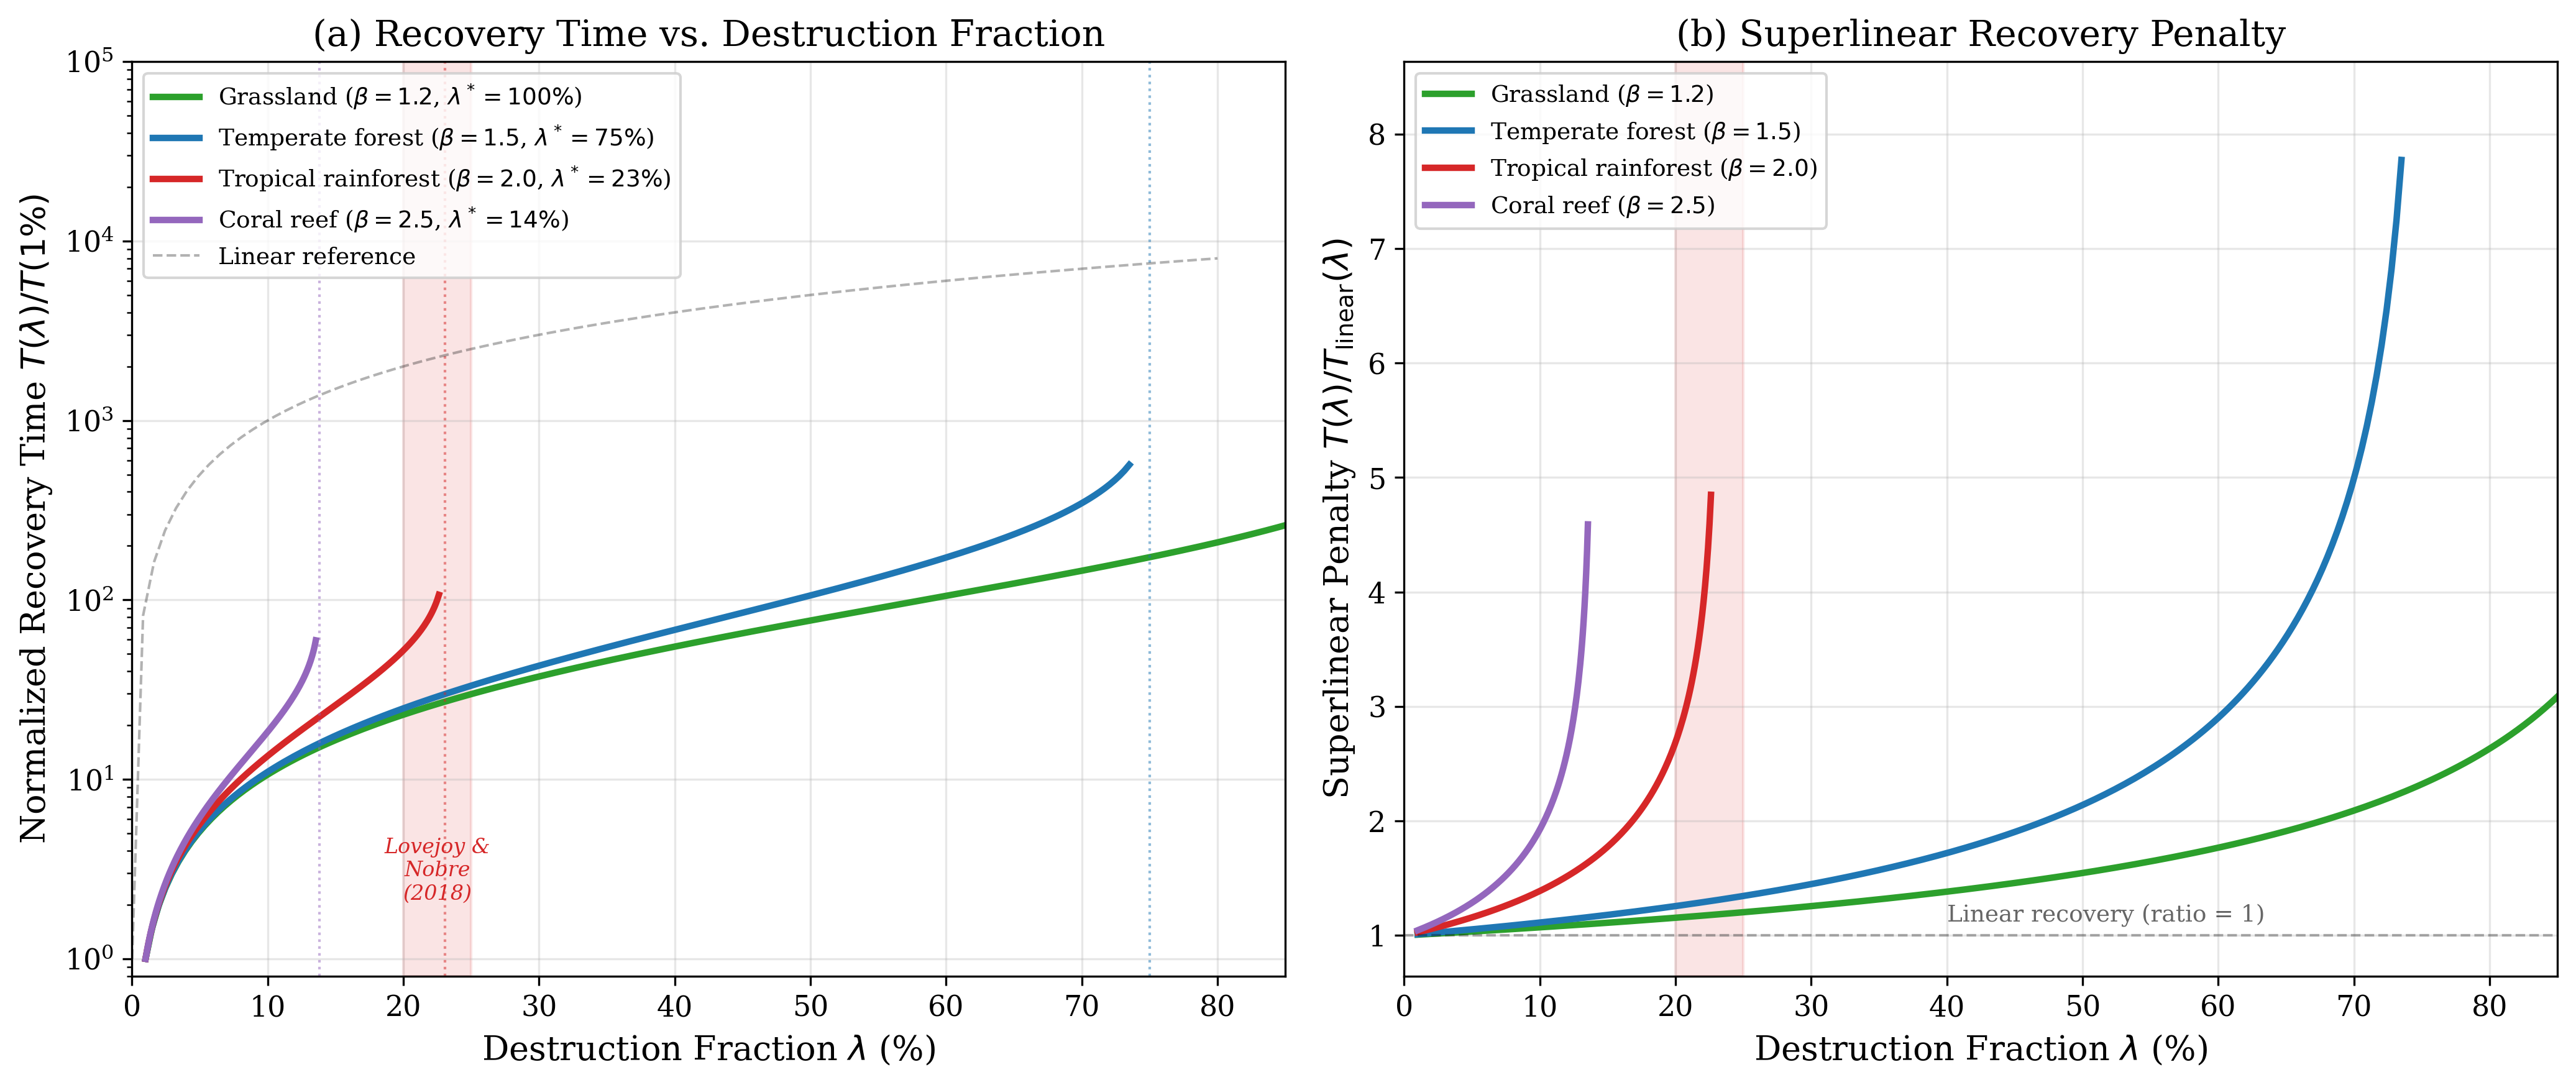
\includegraphics[keepaspectratio,alt={Figure 8: Superlinear Recovery Time. (a) Normalized recovery time T(\textbackslash lambda)/T(1\textbackslash\%) vs.~destruction fraction \textbackslash lambda for four ecosystem types with different \textbackslash beta values and surplus ratios. Grasslands (\textbackslash beta = 1.2) show approximately linear recovery; tropical rainforests (\textbackslash beta = 2.0) and coral reefs (\textbackslash beta = 2.5) show sharply nonlinear recovery diverging at the tipping threshold \textbackslash lambda\^{}*. The shaded band marks the Lovejoy-Nobre 20-25\% Amazon threshold. (b) Superlinear penalty ratio T(\textbackslash lambda)/T\_\{\textbackslash text\{linear\}\}(\textbackslash lambda): a ratio of 1 indicates linear recovery; values exceeding 1 indicate superlinear time debt. High-\textbackslash beta systems incur steeply increasing time penalties with each additional percent of destruction.}]{fig_recovery_time.png}}
\caption{Figure 8: Superlinear Recovery Time. (a) Normalized recovery
time \(T(\lambda)/T(1\%)\) vs.~destruction fraction \(\lambda\) for four
ecosystem types with different \(\beta\) values and surplus ratios.
Grasslands (\(\beta = 1.2\)) show approximately linear recovery;
tropical rainforests (\(\beta = 2.0\)) and coral reefs (\(\beta = 2.5\))
show sharply nonlinear recovery diverging at the tipping threshold
\(\lambda^*\). The shaded band marks the Lovejoy-Nobre 20-25\% Amazon
threshold. (b) Superlinear penalty ratio
\(T(\lambda)/T_{\text{linear}}(\lambda)\): a ratio of 1 indicates linear
recovery; values exceeding 1 indicate superlinear time debt.
High-\(\beta\) systems incur steeply increasing time penalties with each
additional percent of destruction.}
\end{figure}

\subsection{The Conservation Fidelity
Bound}\label{the-conservation-fidelity-bound}

A natural proposal for mitigating destruction is \emph{ex-situ
conservation}: copying the information content of a complex system
(genome databases, seed banks, tissue archives) before allowing the
original to be destroyed. The following result establishes that this
strategy faces a fundamental thermodynamic limitation: the cost of
maintaining functional fidelity in an ex-situ copy converges to the cost
of maintaining the system in situ.

\begin{definition}[Static Information]
\label{def-static-information}

The \textbf{static information} $H_{\text{static}}$ of a complex dissipative structure $S$ is the component of its total functional information consisting of sequence data, molecular blueprints, and structural specifications that can be encoded as a bit string and copied at Landauer cost $W_L = H_{\text{static}} \cdot k_B T \ln 2$. Examples: genome sequences, protein primary structures, morphological descriptions.
\end{definition}

\begin{definition}[Dynamic Information]
\label{def-dynamic-information}

The \textbf{dynamic information} $H_{\text{dynamic}}$ of a complex dissipative structure $S$ is the component of its total functional information consisting of relational and process information that exists only as ongoing interactions within the system and its environment. Examples: protein folding pathways in cellular context, species interaction networks, epigenetic regulatory states, evolutionary trajectories in adaptive landscapes.

The total functional information decomposes as $H_{\text{func}} = H_{\text{static}} + H_{\text{dynamic}}$.
\end{definition}

\begin{proposition}[Conservation Fidelity Bound]
\label{prop-conservation-fidelity-bound}

Let $S$ be a self-maintaining dissipative structure whose maintenance power $\dot{W}_{\text{maintain}}$ is fully covered by self-captured energy ($\dot{W}_{\text{capture}} \geq \dot{W}_{\text{maintain}}$). Assume that maintaining the dynamic information component $H_{\text{dynamic}}$ (Definition~\ref{def-dynamic-information}) at fidelity $\phi \in [0,1]$ requires reproducing fraction $\phi$ of the internal processes that consume $\dot{W}_{\text{maintain}}$ in the original, so that an ex-situ copy at fidelity $\phi$ has dynamic-maintenance power requirement $\dot{W}_{\text{dyn}}(\phi) \geq \phi \cdot \dot{W}_{\text{maintain}}$. Then the external maintenance power required by the ex-situ copy $S'$ satisfies:

$$\dot{W}_{\text{external}}(\phi) \geq \phi \cdot \dot{W}_{\text{maintain}}$$

since the ex-situ copy, removed from its energy-capture environment, cannot self-maintain.

(a) At $\phi = 0$ (static sequence data only): $\dot{W}_{\text{external}} \approx 0$ (storage cost is negligible: a hard drive consumes far less energy than a living ecosystem).

(b) At $\phi = 1$ (perfect functional replication): $\dot{W}_{\text{external}} \geq \dot{W}_{\text{maintain}}$.

(c) Since $S$ in situ requires zero net external energy (it is self-sustaining), the external cost of ex-situ conservation at fidelity $\phi > 0$ strictly exceeds the external cost of in-situ preservation.
\end{proposition}

\begin{proof}
A self-maintaining dissipative structure satisfies $\dot{W}_{\text{capture}} \geq \dot{W}_{\text{maintain}}$ by definition (this is the condition for thermodynamic self-sustainability). The net external cost of in-situ preservation is therefore $\dot{W}_{\text{in-situ}}^{\text{ext}} = \max(0,\, \dot{W}_{\text{maintain}} - \dot{W}_{\text{capture}}) = 0$.

For an ex-situ copy at fidelity $\phi$: by hypothesis, maintaining the dynamic information at fidelity $\phi$ requires reproducing fraction $\phi$ of the internal processes that consume $\dot{W}_{\text{maintain}}$ in the original. Since the copy is removed from the self-capture environment, $\dot{W}_{\text{capture}}^{S'} \approx 0$ for a synthetic archive; therefore all maintenance energy must be supplied externally, giving $\dot{W}_{\text{external}}(\phi) \geq \phi \cdot \dot{W}_{\text{maintain}}$. Parts (a) and (b) follow by substitution. For (c): for any $\phi > 0$, $\dot{W}_{\text{external}}(\phi) \geq \phi \cdot \dot{W}_{\text{maintain}} > 0 = \dot{W}_{\text{in-situ}}^{\text{ext}}$, a strict inequality.
\end{proof}

\begin{corollary}[Generative Loss of Ex-Situ Copies]
\label{cor-generative-loss-ex-situ}

An ex-situ copy at fidelity $\phi < 1$ also forfeits a fraction $(1 - \phi)$ of the original system's generative information stream. Under rate-stock coupling, the capitalized value of this lost stream is:

$$\Delta PV_{\text{gen}}(\phi) = \frac{\alpha v \mathcal{N}^\beta}{r}[1 - \phi^\beta]$$

which exceeds $(1-\phi)$ of the total generative value for $\beta > 1$: even small fidelity losses produce disproportionately large generative-value losses.
\end{corollary}

\begin{proof}
The ex-situ copy's effective negentropy is $\phi \mathcal{N}$, giving generative rate $\alpha(\phi\mathcal{N})^\beta = \alpha\phi^\beta\mathcal{N}^\beta$. The loss relative to the original is $\alpha\mathcal{N}^\beta(1 - \phi^\beta)$, capitalized at rate $r$. Since $\phi^\beta < \phi$ for $\phi \in (0,1)$ and $\beta > 1$, we have $1 - \phi^\beta > 1 - \phi$.
\end{proof}

\begin{remark}[Implications for conservation strategy]
\label{rem-conservation-strategy}

Proposition~\ref{prop-conservation-fidelity-bound} and Corollary~\ref{cor-generative-loss-ex-situ} together formalize a principle well understood by conservation biologists: ex-situ archives (seed banks, genome databases, frozen tissue repositories) are complements to in-situ habitat preservation, not substitutes for it. A genome sequence ($\phi \approx 0$: static information only) is cheap to store but preserves almost none of the system's dynamic or generative value. Maintaining a living population in a controlled environment ($\phi$ moderate) recovers some dynamic information but at non-trivial ongoing cost. Only full in-situ preservation ($\phi = 1$) captures the complete generative stream at zero net external cost, precisely because the self-sustaining dissipative structure pays its own maintenance from captured environmental energy. These results provide a thermodynamic basis for the precautionary principle in conservation: when in doubt, preserve in situ.
\end{remark}

\section{Synthesis: The Cross-Scale Sustainability
Theorem}\label{synthesis-the-cross-scale-sustainability-theorem}

\subsection{Synthesizing the Bounds}\label{synthesizing-the-bounds}

Combining the results of this section:

\begin{theorem}[Cross-Scale Sustainability Theorem]
\label{thm-negentropy-defense}

For a complex dissipative structure, three independent thermodynamic bounds establish that the costs of destruction exceed its yields:

(i) \textbf{Stock bound:} The accumulated negentropy $\mathcal{N}_{\text{bio}} \sim 10^{29}$ J exceeds the net destruction yield $E_{\text{destroy}} - W_{\text{destroy}} \sim 10^{22}$ J by a factor of $\sim 10^7$ (Theorem~\ref{thm-irrationality-destruction}).

(ii) \textbf{Flow bound:} The biosphere's generative information rate $\dot{\mathcal{I}}_{\text{gen}} > 0$ constitutes a perpetual stream of novel information with present value $PV_{\text{gen}} = \dot{\mathcal{I}}_{\text{gen}} \cdot v / r$, which is permanently lost upon destruction (Theorem~\ref{thm-present-value-generative-info}). Under rate-stock coupling (Proposition~\ref{prop-superlinear-destruction-penalty}), even partial destruction degrades this stream superlinearly.

(iii) \textbf{Friction bound:} Dismantling a distributed adaptive biosphere requires sustained boundary-breaking at cost $W_{\text{destroy}} \geq 10^{18}$ J and injects thermodynamic friction into every connected network, degrading downstream operational efficiency (Theorem 10 \citep{TC-IV}).

Two of these three bounds (flow, friction) are independent of how the system's complexity is valued.
\end{theorem}

\begin{proof}
We verify each bound independently.

\textbf{Stock bound:} $E_{\text{destroy}} - W_{\text{destroy}} \approx 10^{22}$ J (Proposition~\ref{prop-minimum-destruction-energy}). The accumulated negentropy lost is $\mathcal{N} \sim 10^{29}$ J (Theorem~\ref{thm-minimum-replication-cost}, Estimate 1). Since $10^{22} \ll 10^{29}$, the energy recovered does not compensate for the information destroyed (Theorem~\ref{thm-irrationality-destruction}). ✓

\textbf{Flow bound:} Destruction eliminates a positive-NPV stream of novel information (Theorem~\ref{thm-present-value-generative-info}). A self-maintaining biosphere captures this stream at zero external cost. ✓

\textbf{Friction bound:} Large-scale destruction injects friction $\Delta\phi = \eta \cdot W_{\text{destroy}}$ (Definition 8 \citep{TC-IV}) with total cascading cost $\eta \cdot W_{\text{destroy}} \cdot M \bar{E} / \epsilon$ over the full recovery period (Theorem 10 \citep{TC-IV}), degrading all connected networks (Theorem 4 \citep{TC-V}). ✓

By the valuation-independent bounds (§\ref{robustness-valuation-independent-bounds}), the flow and friction bounds are independent of how the system's complexity is valued.
\end{proof}

\section{Worked Examples}\label{worked-examples}

\subsection{Example 1: Single Genome, Random Assembly
vs.~Evolution}\label{example-1-single-genome-random-assembly-vs.-evolution}

\textbf{Question:} What is the probability that random assembly produces
a functional human genome?

\textbf{Setup:} The human genome has
\(\mathcal{I}_{\text{func}} = 6.4 \times 10^8\) functional bits. Each
bit must be correct for the genome to be functional (conservative:
binary choice per position).

\textbf{Probability of random success:}

\[p_{\text{random}} = 2^{-\mathcal{I}_{\text{func}}} = 2^{-6.4 \times 10^8} \approx 10^{-1.93 \times 10^8}\]

\textbf{Expected trials needed:}
\(1/p_{\text{random}} \approx 10^{1.93 \times 10^8}\) trials.

\textbf{Minimum energy per trial} (Landauer bound):
\(\mathcal{I}_{\text{func}} \times k_B T \ln 2 = 6.4 \times 10^8 \times 2.87 \times 10^{-21} = 1.84 \times 10^{-12}\)
J.

\textbf{Total expected minimum energy:}

\[W_{\text{random}} = 10^{1.93 \times 10^8} \times 1.84 \times 10^{-12} \approx 10^{1.93 \times 10^8} \text{ J}\]

For comparison, the observable universe contains approximately
\(10^{69}\) J of energy\citep{Penrose2005}. The random-assembly cost
exceeds the energy content of the observable universe by a factor of
\(\sim 10^{1.93 \times 10^8 - 69} \approx 10^{1.93 \times 10^8}\).
Random assembly of a functional genome is not merely impractical; it is
cosmically impossible.

\textbf{What evolution achieves:} By using selection pressure to retain
favorable mutations incrementally, evolution reduces the search cost
from \(\sim 10^{1.93 \times 10^8}\) J (random) to \(\sim 10^{29}\) J
(the accumulated negentropy of the biosphere). This is a search
efficiency factor of
\(\sigma \approx 10^{29} / 10^{1.93 \times 10^8} \approx 10^{-1.93 \times 10^8 + 29}\),
illustrating why evolution, despite appearing ``wasteful,'' is an
extraordinarily efficient search algorithm relative to blind random
search.

\subsection{Example 2: Accumulated Negentropy vs.~Human Energy
Use}\label{example-2-accumulated-negentropy-vs.-human-energy-use}

\textbf{Question:} How does the biosphere's accumulated negentropy
compare to the scale of human economic activity?

\textbf{Setup:}

{\def\LTcaptype{none} % do not increment counter
\begin{longtable}[]{@{}
  >{\raggedright\arraybackslash}p{(\linewidth - 4\tabcolsep) * \real{0.3333}}
  >{\raggedright\arraybackslash}p{(\linewidth - 4\tabcolsep) * \real{0.3333}}
  >{\raggedright\arraybackslash}p{(\linewidth - 4\tabcolsep) * \real{0.3333}}@{}}
\toprule\noalign{}
\begin{minipage}[b]{\linewidth}\raggedright
Quantity
\end{minipage} & \begin{minipage}[b]{\linewidth}\raggedright
Value
\end{minipage} & \begin{minipage}[b]{\linewidth}\raggedright
Source
\end{minipage} \\
\midrule\noalign{}
\endhead
\bottomrule\noalign{}
\endlastfoot
Biosphere accumulated negentropy \(\mathcal{N}_{\text{bio}}\) &
\(\sim 10^{29}\) J &
§\ref{top-down-solar-energy-captured-by-the-biosphere} \\
Global primary energy consumption (2024) & \(\sim 6 \times 10^{20}\)
J/yr & IEA World Energy Outlook \\
Cumulative human energy use over all of history (\(\sim 10^4\) yrs) &
\(\sim 10^{23}\) J & See note below \\
\end{longtable}
}

\emph{Note on cumulative estimate:} Industrial-era consumption
($\sim$200 years averaging \(\sim 5 \times 10^{12}\) W) contributes
\(\sim 3 \times 10^{22}\) J. Pre-industrial consumption (\(\sim 10^4\)
years at \(\sim 10^{11}\) W) contributes a comparable amount. The sum
lies in the range \(3 \times 10^{22}\) to \(3 \times 10^{23}\) J; we use
\(\sim 10^{23}\) J as a round upper bound.

The biosphere's accumulated negentropy exceeds cumulative human energy
consumption over all of recorded history by a factor of \(\sim 10^6\).
Even if global energy consumption continued at current rates for another
million years, the total (\(\sim 6 \times 10^{26}\) J) would still fall
short of \(\mathcal{N}_{\text{bio}}\) by two orders of magnitude.

\textbf{The search cost is the binding constraint.} The search cost
amplification factor \(\Xi \sim 10^{35}\)
(Definition~\ref{def-search-cost-amplification}) means that the
evolutionary process that discovered \emph{which} configurations are
functional consumed \(10^{35}\) times more energy than the Landauer
minimum for writing the resulting information. Raw energy is not the
bottleneck for replacing biological complexity; the bottleneck is the
search cost of rediscovering \(\sim 10^{15}\) bits of functional
information from a configuration space of size
\(\sim 10^{6.4 \times 10^8}\).

\textbf{Conclusion:} The biosphere's accumulated thermodynamic
investment dwarfs the total energy throughput of human civilization. The
information it encodes, selected over \(4 \times 10^9\) years of
evolutionary search, represents the single most information-dense
structure in the known Solar System.

\subsection{Example 3: The Burning-Library
Quantification}\label{example-3-the-burning-library-quantification}

The Burning-Library Ratio (Definition~\ref{def-burning-library-ratio})
quantifies the fraction of a system's accumulated thermodynamic
investment recoverable through destruction. The following worked
examples compute this ratio at two scales: a single ecosystem and the
full biosphere.

\subsubsection{The Amazon Rainforest}\label{the-amazon-rainforest}

\textbf{Question:} What fraction of the Amazon's accumulated
thermodynamic value is recovered by converting its biomass to raw
energy?

\textbf{Setup:}

{\def\LTcaptype{none} % do not increment counter
\begin{longtable}[]{@{}
  >{\raggedright\arraybackslash}p{(\linewidth - 4\tabcolsep) * \real{0.3333}}
  >{\raggedright\arraybackslash}p{(\linewidth - 4\tabcolsep) * \real{0.3333}}
  >{\raggedright\arraybackslash}p{(\linewidth - 4\tabcolsep) * \real{0.3333}}@{}}
\toprule\noalign{}
\begin{minipage}[b]{\linewidth}\raggedright
Quantity
\end{minipage} & \begin{minipage}[b]{\linewidth}\raggedright
Value
\end{minipage} & \begin{minipage}[b]{\linewidth}\raggedright
Source
\end{minipage} \\
\midrule\noalign{}
\endhead
\bottomrule\noalign{}
\endlastfoot
Total biomass (above and below-ground) & 86 Pg C &
\citet{Saatchi2007} \\
Dry mass (\(2\times\) carbon conversion) & \(1.72 \times 10^{14}\) kg &
Calculated \\
Calorific value (tropical hardwood) & \(\sim 19\) MJ/kg & Standard
thermodynamic value \\
Amazon basin GPP & \(\sim 20\) Pg C/yr &
\citet{SciencePanelAmazon2021} \\
Global terrestrial GPP & \(\sim 120\) Pg C/yr & \citet{Beer2010} \\
\end{longtable}
}

\textbf{Extractable energy.} The Amazon basin contains approximately 86
Pg C of total biomass \citep{Saatchi2007}, corresponding to
\(\sim 1.72 \times 10^{14}\) kg of dry mass. At a calorific value of
\(\sim 19\) MJ/kg for tropical hardwood:

\[E_{\text{destroy}} \approx 1.72 \times 10^{14} \times 1.9 \times 10^{7} \approx 3.3 \times 10^{21} \text{ J}\]

\textbf{Accumulated negentropy (lower bound).} The Amazon contributes
approximately 16\% of global terrestrial gross primary production
(\(\sim 20\) out of \(\sim 120\) Pg C/yr;
\citet{SciencePanelAmazon2021}; \citet{Beer2010}). Allocating biosphere
accumulated negentropy
(§\ref{top-down-solar-energy-captured-by-the-biosphere}) in proportion
to productivity share:

\[\mathcal{N}_{\text{Amazon}} \sim \frac{P_{\text{GPP, Amazon}}}{P_{\text{GPP, global}}} \cdot \mathcal{N}_{\text{bio}} \approx 0.16 \times 10^{29} \sim 10^{28} \text{ J}\]

This is a lower bound: the Amazon is disproportionately biodiverse
relative to its productivity share, and the underlying biosphere
estimate uses a conservative ordering efficiency
(\(\eta_{\text{order}} = 0.01\)). The modern Amazon basin has sustained
continuous tropical forest cover for at least \(5.5 \times 10^7\) years
\citep{Morley2000}, but the lineages it shelters inherit metabolic and
informational complexity accumulated over the full
\(4 \times 10^9\)-year history of life.

\textbf{Burning-Library Ratio:}

\[\mathcal{R}_{\text{BL}} = \frac{E_{\text{destroy}}}{\mathcal{N}_{\text{Amazon}}} = \frac{3.3 \times 10^{21}}{10^{28}} \approx 3 \times 10^{-7}\]

\textbf{Result:} Complete destruction of the Amazon rainforest recovers
approximately three ten-millionths of its accumulated thermodynamic
value as raw energy. The remaining 99.99997\% represents information and
structural complexity that destruction dissipates irreversibly. This
ratio is comparable to the biosphere-scale result computed below.

\subsubsection{Earth's Biosphere}\label{earths-biosphere}

\textbf{Question:} What fraction of the biosphere's value is recovered
by harvesting its raw chemical energy?

\textbf{Setup:} - Extractable chemical energy:
\(E_{\text{destroy}} \sim 10^{22}\) J (§\ref{the-destruction-yield}) -
Accumulated negentropy: \(\mathcal{N}_{\text{bio}} \sim 10^{29}\) J
(§\ref{top-down-solar-energy-captured-by-the-biosphere}) - Generative
information value (100-year horizon, \(r = 0.05\)):
\(PV_{\text{gen}} = \dot{\mathcal{I}}_{\text{gen}} \cdot v / r\)

Estimating the generative rate: global speciation rate \(\sim 10^{-3}\)
to \(10^{-1}\) new species per year across all taxa, each contributing
\(\sim 10^7\) unique bits, giving
\(\dot{\mathcal{I}}_{\text{gen}} \sim 10^4\) to \(10^6\) bits/yr. At
\(v \sim 10^9\) J/bit (order-of-magnitude cost of producing one
functional bit through evolution, from
\(\mathcal{N}_{\text{bio}} / H_{\text{biosphere}} \approx 10^{29}/10^{15} = 10^{14}\)
J/bit, however we use \(v \sim 10^9\) as a conservative valuation
reflecting diminishing marginal returns):

\[PV_{\text{gen}} \sim \frac{10^6 \times 10^9}{0.05} = 2 \times 10^{16} \text{ J}\]

\textbf{Total preservation value:}

\[V_{\text{preserve}} = \mathcal{N}_{\text{bio}} + PV_{\text{gen}} \approx 10^{29} + 10^{16} \approx 10^{29} \text{ J}\]

(The stock term dominates.)

\textbf{Fraction recovered by destruction:}

\[\frac{E_{\text{destroy}}}{V_{\text{preserve}}} = \frac{10^{22}}{10^{29}} = 10^{-7}\]

\textbf{Result:} The extractable raw energy from the biosphere is one
ten-millionth of its total thermodynamic value. The remaining 99.99999\%
of the accumulated investment has no recoverable energy equivalent.

\section{Discussion}\label{discussion}

\subsection{Physical Interpretation}\label{physical-interpretation}

The accumulated negentropy framework provides a thermodynamic accounting
of irreversibility in complex systems. The central result, the
Burning-Library Ratio of \(\sim 10^{-7}\)
(Corollary~\ref{cor-burning-library-inequality}), quantifies the gap
between the energy extractable through destruction and the thermodynamic
investment embodied in biological complexity. This is not a subjective
valuation but a physical accounting: the work required to recreate the
information content exceeds the energy recoverable from destruction by
seven orders of magnitude.

The biosphere estimate of \(\mathcal{N}_{\text{bio}} \sim 10^{29}\) J is
cross-validated by an independent calculation using Chaisson's energy
rate density measurements \citep{Chaisson2011} weighted by Bar-On et
al.'s biomass fractions \citep{BarOn2018}, which yields
\(\sim 7 \times 10^{28}\) J
(§\ref{cross-validation-via-energy-rate-density}). Agreement within a
factor of 1.36 between two methodologically independent routes (solar
flux accounting vs.~organism-level energy budgets) provides robust
confirmation of the order of magnitude.

The result is robust to substantial parameter uncertainty
(\ref{rem-order-of-magnitude}). Even if the accumulated negentropy
estimate is wrong by a factor of \(10^3\), the gap remains four orders
of magnitude. The Burning-Library Ratio provides a physically grounded,
order-of-magnitude ``floor'' on the value of complex systems.

The cost-benefit bound (Theorem~\ref{thm-irrationality-destruction}) and
the cross-scale sustainability theorem
(Theorem~\ref{thm-negentropy-defense}) together establish three
independent thermodynamic bounds on the costs of destruction: stock
value, generative information flow, and network friction costs.
Crucially, two of these three bounds are valuation-independent
(§\ref{robustness-valuation-independent-bounds}): the flow and friction
bounds impose costs regardless of the purpose of the extraction. The
convergence of these independent bounds makes the conclusion robust to
failure of any single bound: even if one metric were invalidated, the
remaining two suffice.

The rate-stock coupling framework (§\ref{the-generative-data-argument})
adds dynamic consequences to the static Burning-Library accounting. The
front-loaded cost structure
(Proposition~\ref{prop-portfolio-destruction-ordering}) shows that the
marginal cost of destruction is highest for the first increment,
creating a strong thermodynamic disincentive against initiating any
damage. Recovery from destruction is superlinear in the damage fraction
(Proposition~\ref{prop-superlinear-recovery-time}): doubling the
destruction more than doubles the recovery time, and recovery diverges
to infinity at the tipping threshold. The conservation fidelity bound
(Proposition~\ref{prop-conservation-fidelity-bound}) establishes that
ex-situ archives (seed banks, genome databases) are complements to, not
substitutes for, in-situ preservation, because the external cost of
maintaining dynamic information at high fidelity converges to the
in-situ maintenance cost while the original self-maintains at zero
external cost.

\subsection{Testable Predictions}\label{testable-predictions}

These results generate falsifiable predictions:

{\def\LTcaptype{none} % do not increment counter
\begin{longtable}[]{@{}
  >{\raggedright\arraybackslash}p{(\linewidth - 4\tabcolsep) * \real{0.3333}}
  >{\raggedright\arraybackslash}p{(\linewidth - 4\tabcolsep) * \real{0.3333}}
  >{\raggedright\arraybackslash}p{(\linewidth - 4\tabcolsep) * \real{0.3333}}@{}}
\toprule\noalign{}
\begin{minipage}[b]{\linewidth}\raggedright
Prediction
\end{minipage} & \begin{minipage}[b]{\linewidth}\raggedright
Source
\end{minipage} & \begin{minipage}[b]{\linewidth}\raggedright
Falsified If\ldots{}
\end{minipage} \\
\midrule\noalign{}
\endhead
\bottomrule\noalign{}
\endlastfoot
Biosphere accumulated negentropy \(\sim 10^{29}\) J &
Definition~\ref{def-accumulated-negentropy},
§\ref{biosphere-estimation-the-4-billion-year-ledger} estimates &
Independent estimates of ordering work over geological time yield
\(< 10^{26}\) J or \(> 10^{32}\) J \\
Cross-validation via Chaisson's \(\Phi_m\) yields
\(\sim 7 \times 10^{28}\) J &
§\ref{cross-validation-via-energy-rate-density}, \citep{Chaisson2011} &
Organism-level energy budgets yield biosphere ordering rate inconsistent
with GPP by more than an order of magnitude \\
Burning-Library Ratio \(\sim 10^{-7}\) for Earth's biosphere &
Corollary~\ref{cor-burning-library-inequality} & Extractable chemical
energy from biomass exceeds \(10^{26}\) J, or accumulated negentropy is
below \(10^{26}\) J \\
Generative information rate \(\dot{\mathcal{I}}_{\text{gen}} > 0\) for
evolving ecosystems & Theorem~\ref{thm-present-value-generative-info} &
An active biosphere produces no novel functional information over
measurable timescales (no speciation, no adaptive mutations) \\
Replication cost \(\geq \mathcal{N}_{\text{bio}}\) for blind-search
rebuilding & Theorem~\ref{thm-minimum-replication-cost} & A demonstrated
method reconstructs an equivalently complex information-bearing system
at energy cost \(\ll \mathcal{N}\) \\
Superlinear generative-value loss under partial destruction &
Proposition~\ref{prop-superlinear-destruction-penalty} & Empirical
measurement of speciation or adaptive mutation rates in ecosystems of
varying complexity shows a linear (not superlinear) relationship between
complexity and generative rate \\
Tipping threshold \(\lambda^*\) consistent with Lovejoy-Nobre 20-25\% &
Proposition~\ref{prop-negentropy-tipping-point},
\citep{LovejoyNobre2018} & Calibrated \(\beta\) and \(R\) for the Amazon
yield \(\lambda^*\) outside the 15-30\% range, or grasslands show
comparable threshold fragility \\
Recovery time convex in destruction fraction, diverging at \(\lambda^*\)
& Proposition~\ref{prop-superlinear-recovery-time} & Ecosystem recovery
timescales scale linearly with damage fraction, or severely damaged
high-\(\beta\) systems recover as fast as low-\(\beta\) systems \\
Ex-situ conservation cost converges to in-situ cost at high fidelity &
Proposition~\ref{prop-conservation-fidelity-bound} & Maintaining a
functionally complete ex-situ replica of a complex ecosystem at
substantially lower energy cost than the original \\
\end{longtable}
}

\subsection{Limitations}\label{limitations}

The accumulated negentropy results depend on order-of-magnitude
estimates that are robust to factor-of-10 uncertainties but sensitive to
definitions of ``functional information'' (see
\ref{rem-order-of-magnitude}). The distinction between total Shannon
entropy and functionally relevant information remains an active research
question. The Burning-Library Ratio's seven-order-of-magnitude gap
provides substantial margin against this definitional uncertainty: even
factor-of-\(10^3\) errors in the accumulated negentropy estimate leave a
four-order-of-magnitude gap.

The search cost amplification factor (\(\Xi \sim 10^{35}\)) assumes
blind search as the baseline. Directed search methods (evolution,
machine learning) reduce this, but even optimistic estimates leave the
amplification at \(\sim 10^{10}\) to \(10^{20}\).

The rate-stock coupling (Definition~\ref{def-rate-stock-coupling},
Proposition~\ref{prop-superlinear-destruction-penalty}) assumes a
power-law functional form
\(\dot{\mathcal{I}}_{\text{gen}} = \alpha \mathcal{N}^\beta\) with
\(\beta > 1\). The superlinearity is motivated by the combinatorial
argument (more components yield superlinearly more interaction
possibilities), but the exponent \(\beta\) has not been directly
measured. However, the tipping-point prediction
(Proposition~\ref{prop-negentropy-tipping-point}) provides an indirect
calibration: the observed 20-25\% deforestation threshold for the Amazon
\citep{LovejoyNobre2018} implies a generative surplus ratio
\(R \approx 1.25\)-\(1.33\), and the contrast between
threshold-dominated tropical forests and resilient grasslands is
consistent with \(\beta \approx 2\) for the former and
\(\beta \approx 1.2\) for the latter. Direct ecological measurement of
the relationship between ecosystem complexity and information generation
rate would test the superlinearity assumption and constrain \(\beta\);
the analysis predicts that this relationship is steepest for
species-rich systems with dense interaction networks.

\textbf{Scope.} The results apply to any complex dissipative system
whose information content was produced by an extended search process
(evolutionary, developmental, or cultural). The biosphere estimation in
§\ref{biosphere-estimation-the-4-billion-year-ledger} uses
Earth-specific parameters, but the formal results
(Theorem~\ref{thm-irrationality-destruction},
Theorem~\ref{thm-negentropy-defense}) hold for any system satisfying the
assumptions of §\ref{model-and-formal-setup}. This analysis does not
address the \emph{distribution} of value within the biosphere (whether
individual species or ecosystems are equally irreplaceable); such
distributional questions require finer-grained estimates of
per-subsystem accumulated negentropy.

\subsection{Applications}\label{applications}

\textbf{Conservation economics.} The Burning-Library Ratio provides a
computable standard for preservation policy: the thermodynamic cost of
replacing a destroyed ecosystem can be compared against the economic
value of the resources extracted. For any ecosystem with accumulated
negentropy \(\mathcal{N}\) and extractable resource value
\(E_{\text{extract}}\), the ratio \(E_{\text{extract}} / \mathcal{N}\)
quantifies the fraction of accumulated value recoverable through
destruction. Where this ratio is small (as it is for all biologically
complex systems), destruction is a net-negative trade even before
accounting for ecosystem services. In
§\ref{example-3-the-burning-library-quantification}, the ratio has been
computed for the Amazon rainforest
(\(\mathcal{R}_{\text{BL}} \sim 10^{-7}\)) in addition to the full
biosphere, confirming that the seven-order-of-magnitude gap persists at
the individual ecosystem scale.

\textbf{Cultural and institutional capital.} The analysis applies to any
complex dissipative system whose information content was produced by
extended search (§\ref{model-and-formal-setup}). Cultural systems
(languages, legal traditions, indigenous knowledge) are plausible
candidates: their information content was refined over generations
through iterative selection, and they are maintained through continued
use. Whether the Burning-Library Ratio and rate-stock coupling results
transfer quantitatively to such systems is an open empirical question,
but the formal structure suggests that the asymmetry between destruction
cost and reconstruction cost may be similarly severe wherever the
underlying information was produced by extended trial-and-error rather
than deliberate design.

\textbf{Information thermodynamics.} The search cost amplification
factor \(\Xi\) (Definition~\ref{def-search-cost-amplification})
quantifies the gap between the Landauer floor and the actual cost of
producing functional information through evolutionary search. This
quantity is of independent interest in information thermodynamics, since
it measures the computational work embodied in a specific
information-bearing configuration, a concept with potential applications
in quantifying the value of databases, cultural knowledge, and other
complex information systems.

\subsection{Future Work}\label{future-work}

\textbf{Sub-biosphere calibration.} Developing detailed estimates of
\(\mathcal{N}(T)\) for ecosystems at multiple scales (individual
organisms, local ecosystems, regional biomes) would empirically validate
the analysis and provide calibration data for the Burning-Library Ratio
at sub-biosphere scales. Genome-level validation of the information
density hierarchy (Definition~\ref{def-information-density},
Definition~\ref{def-specific-information-density}) against molecular
evolution data would test the bottom-up estimation methodology.

\textbf{Rate-stock coupling measurement.} Direct empirical calibration
of the rate-stock coupling exponent \(\beta\)
(Definition~\ref{def-rate-stock-coupling}) from comparative data on
speciation rates and ecosystem complexity would provide a quantitative
test of the superlinearity assumption. The tipping-point observations in
§\ref{the-generative-data-argument} provide indirect constraints
(\(\beta \approx 2\) for tropical forests, \(\beta \approx 1.2\) for
grasslands), but systematic measurement across diverse system types is
needed.

\textbf{Independent cross-validation.} Extending the Chaisson
cross-validation (§\ref{cross-validation-via-energy-rate-density}) to
include independent estimates from geochemistry and population genetics
would further constrain the biosphere negentropy estimate.

\textbf{Dynamic negentropy accumulation in production networks.}
Accumulated negentropy is defined here as a stock. A dynamic extension
to production networks would formalize the \emph{flow} that builds it:
integrated net production over evolutionary time, constrained by
thermodynamic admissibility. Recovery from collapse would acquire a
formal criterion (the spectral radius of the remaining production
network must remain below one and the Hawkins-Simon condition must hold
on the residual input-output matrix). The Burning-Library Ratio would
become the static limit of a dynamic irreplaceability result.

\textbf{Conditional replacement cost.} The blind search replication cost
(Theorem~\ref{thm-minimum-replication-cost}) assumes reconstruction from
zero prior information, yielding the amplification factor
\(\Xi \sim 10^{35}\). When phylogenetic or informational neighbors of
the destroyed system survive, they provide a template that reduces the
effective search space. A conditional replacement cost
\(\Xi_{\text{eff}}\), discounted by the mutual information between the
destroyed system and the best surviving template, would formalize this
reduction:
\(\Xi_{\text{eff}} = \Xi \cdot 2^{-I(\text{destroyed};\text{template})}\).
For closely related species sharing $>$95\% genomic identity, the
discount could span tens of orders of magnitude. The blind search bound
remains tight only when the destroyed system is truly unique (no close
relatives, no archived information).

\section{Conclusion}\label{conclusion}

We have defined accumulated negentropy as the integrated thermodynamic
work embodied in complex dissipative structures and computed the
Burning-Library Ratio at biosphere scale: the fraction of accumulated
value recoverable through destruction. For Earth's biosphere, this ratio
is approximately \(10^{-7}\), a gap of seven orders of magnitude that is
robust to substantial parameter uncertainty and cross-validated within a
factor of 1.36 by independent energy rate density measurements
(§\ref{cross-validation-via-energy-rate-density}). Living systems
generate information at a positive rate whose present value is
unbounded; under the rate-stock coupling formalized here, even partial
destruction incurs a superlinear penalty on future information
production.

The dynamic consequences of rate-stock coupling extend the static
Burning-Library accounting. Complex systems with high coupling exponents
(\(\beta \gg 1\)) exhibit tipping-point fragility: the Amazon's 20-25\%
deforestation threshold \citep{LovejoyNobre2018} is consistent with the
predicted tipping fraction \(\lambda^*\) for a system operating
$\sim$25-33\% above its maintenance threshold. Recovery from
sub-threshold damage is superlinear in the damage fraction, explaining
why grasslands (\(\beta \approx 1.2\)) recover in years while tropical
forests (\(\beta \approx 2\)) require centuries, if they recover at all.
The front-loaded cost structure of destruction means that an intact
ecosystem's first increment of damage is the most expensive. Ex-situ
conservation archives capture only static information; maintaining
dynamic fidelity converges in cost to maintaining the original system,
while the original self-maintains at zero external cost.

Both thermodynamic bounds beyond the stock bound are
valuation-independent (§\ref{robustness-valuation-independent-bounds}).
Together, these results establish computable, energy-denominated
sustainability limits for any complex dissipative structure whose
information content was produced by extended search.

These results require only Landauer's principle and basic
thermodynamics. They provide the irreplaceability component of the
multi-agent cooperation models developed in \emph{Necessary Constraints}
\citep{TC-I} and \emph{Thermodynamic Friction} \citep{TC-IV}. The
strategic entropy injection analysis \citep{TC-II} addresses information
corruption costs at the agent-to-agent level; the present paper extends
the information-theoretic analysis to the cross-scale level, quantifying
the irreplaceability of the complex structures that cooperative networks
produce and maintain.

\addcontentsline{toc}{section}{References}
\bibliography{../../shared/main}
\end{document}
